\documentclass[draft]{agujournal2019}

\newcommand{\todo}[1]{\textcolor{red}{\textbf{(#1)}}}

\usepackage{amsmath}

% LTeX: language=en-US

\linenumbers
\journalname{Journal of Advances in Modeling Earth Systems (JAMES)}

\begin{document}

\title{Responses to Humidity and Temperature Perturbations in High-Resolution Simulations of Convection}

\authors{Timothy H. Raupach\affil{1,2,3,4}, Chimene L. Daleu\affil{5}, Robert S.
Plant\affil{5}, Steven C. Sherwood\affil{2,3,4}, and Yi-Ling Hwong\affil{6}}

\affiliation{1}{Institute for Climate Risk and Response, University of New South Wales, Sydney, Australia}
\affiliation{2}{Climate Change Research Centre, University of New South Wales, Sydney, Australia}
\affiliation{3}{ARC Centre of Excellence for Climate Extremes}
\affiliation{4}{ARC Centre of Excellence for 21st Century Weather}
\affiliation{5}{Department of Meteorology, University of Reading, Reading, United Kingdom}
\affiliation{6}{Institute of Science and Technology Austria, Vienna, Austria}

\correspondingauthor{Timothy H. Raupach}{timothy.h.raupach@gmail.com}

\begin{keypoints}
    \item Responses to humidity and temperature perturbations were examined
    using idealised simulations at high resolution for two numerical models.
    \item For the two models examined, accurate simulation of
    convectively-coupled dynamics required a grid spacing of lower than $\sim$1
    km.
    \item The linear responses of LES models with sufficient resolution in these
    idealised tests could reasonably be used as ground truth for Global Climate
    Model scheme testing.
\end{keypoints}

\justifying

\begin{abstract}
Global and regional climate models must take the important effects of
atmospheric convection into account, but are often run at grid spacings at which
convection can not be explicitly modelled. In this case models use convection
schemes to parameterize sub-grid convection and its effects. Convection
parameterization is a leading source of uncertainty in model outputs, and a lack
of ground truth complicates the assessment of convective scheme performance.
Here, we use a linear response framework and show results from perturbation
experiments with two models run at convection-permitting resolution, to attempt
to establish a reference ``truth'' for model responses to temperature and
humidity perturbations. We show that for the models we examined, a grid spacing
of lower than $\sim$1 km was required for accurate representation of
convectively-coupled dynamics. The results from these tests at 100 m and 250 m
grid spacing could reasonably be used as ground truth for scheme testing in
global climate models.
\end{abstract}

\section*{Plain Language Summary}

In the atmosphere, convection is heat-driven movement of air. Convection causes
the rise of buoyant air that forms thunderstorm cells, for example. Convection
forces changes in water state, causing clouds and rain to form, and it also
moves heat around. These effects are so important that weather and climate
models must account for them. A problem arises because models are often run with
grid spacings, or gaps between modelled points, that are larger than the scale
of typical convective cells. In this case, models resort to using simplified
approximations, called convection schemes, to model convection effects in broad
terms and attempt to make up for not explicitly modelling convective cells. It
is difficult to assess the performance of these schemes, because there is no
reliable ground truth that says exactly how the schemes should perform. Here we
study how schemes ``should'' perform by examining how two models react to small
changes in temperature and humidity when they are run at fine-enough resolution
that no convective scheme is required. We show that models require a grid
spacing of under $\sim$1 km to properly capture the effects of convection, and
we propose that the responses we show at the finest resolutions could reasonably
be used as a ground truth for testing of convection schemes.

\section{Introduction}

Global and regional climate models (respectively GCMs and RCMs) must take
convection into account because of its important atmospheric effects
\cite{Manabe_JAS_1964, Wallace_2006}. However, models often use horizontal grid
spacings that are much larger than the horizontal scale of convection, meaning
that they are unable to resolve individual convective cells. In this case, the
model must account for the effects of convection -- such as its heating or the
rain it may produce -- by parameterizing sub-grid convection that it can not
explicitly resolve. Such parameterization methods are called convection schemes. 

Many convection schemes have been produced, each with different strengths,
weaknesses, and assumptions \cite<e.g.>{Arakawa_JC_2004, Rio_CCCR_2019,
Lin_AO_2022}. Such are the differences between these schemes, and so high is the
sensitivity of models to convective cloud physics \cite<e.g.>{Emanuel_JAS_1999},
that convection parameterization is a leading source of uncertainty in model
outputs \cite<e.g.>{Hwong_JAMES_2021}. It is difficult to compare convection
schemes, since traditional methods in which simulated outputs are compared with
observations \cite<e.g.>{Grell_ACP_2014, Kwon_MWR_2017, Zhang_JC_2017,
Zhang_MWR_2011} are limited by observation selection and accuracy (H21).

\citeA{Kuang_JAS_2010}, hereafter K10, suggested that although there are many
non-linear processes in convection, the statistics of the cumulus ensemble as a
whole can be partly described by smooth linear functions that describe how the
ensemble reacts to small changes in its large-scale environment. The
mathematical framework proposed by K10 uses a linear tangent model to
approximate the feedback of small-scale processes on the large-scale
environment, effectively playing the role of a (linear) convective scheme
trained on a large cloud-resolving model (CRM) dataset, such that

\begin{equation} 
\frac{\partial {\bf X}}{\partial t} = {\bf MX},
\end{equation}

\noindent where the partial time derivative represents the feedback on the
column state variable {\bf X}, and {\bf M} is a matrix obtained from perturbed
runs of a cloud-resolving model. In this method, the responses of the model (and
thus the convection scheme) are examined in idealized simulations under
different small perturbations of the humidity and temperature tendencies. K10
provided evidence that these linear responses were sufficient to capture the
dynamics of convectively-coupled waves, which evolve slowly compared to typical
convective response times and have relatively small amplitudes. Even if a linear
approximation is inadequate for fully describing convection for more general
purposes, it can be a useful first-order characterization.

To this end, the linear response framework was applied to single column models
(SCMs) by \citeA{Herman_JAMES_2013}, specifically for the purpose of testing two
convection schemes against the equivalent tangent linear model constructed from
a CRM reference. \citeA{Hwong_JAMES_2021}, hereafter H21, used the framework to
evaluate convection, planetary boundary layer, and microphysics schemes'
responses to perturbations in the SCMs. They showed that the results isolate the
impact of the convection scheme in at least the tested SCMs, and examined many
other schemes in common use. The technique allows for efficient comparison of
different model setups, and \citeA{Herman_JAMES_2013} identified a wide range of
responses among current schemes, showing the potential of the method. However,
the study did not attempt to answer the question of which setup was the most
accurate. To answer this question we need a ``truth'' response, which is not
available from observations. K10 evaluated his linear responses using rather
coarse resolution (2 km)  runs of the System for Atmospheric Modelling
\cite<SAM, e.g.>{Khairoutdinov_JAS_2003}, and in a relatively small domain (128
km square). This resolution would not be considered large-eddy resolving by
today's standards, and the experiment has not been repeated in any other
cloud-resolving model. A study of high-resolution linear responses of a model
that uses the least possible parameterization is therefore required, along with
robustness evaluation.

In this study, we ran perturbation experiments with two different models across
a range of CRM and large eddy simulation (LES) resolutions, seeking to produce
benchmark test results. This enabled us to test the conclusion of H21 that
results are not sensitive to the treatment of the planetary boundary layer (PBL)
for configurations in which convection is resolved explicitly. The key question
is whether the linear responses are robust, or sensitive to decisions made in
high-resolution modelling such as the grid length, model dynamical core, or
treatment of microphysics or eddy mixing. In particular, can we establish a
reference ``truth'' that is less uncertain than the variations between
convection schemes themselves? A second question addressed here, which is
becoming more relevant as we enter an age of global CRMs, is what grid
resolution they would require to properly represent convective-scale feedbacks
on large scale flows -- arguably the key benefit of global CRMs -- and how
sensitive the feedback might be to parameterizations remaining in those models
or to the numerics or other details of the CRM. In summary, here we use CRM and
LES models to address how we should judge the differences between model schemes
reported in H21.

\section{Methods}
\label{sec:methods}

We used two numerical models in this work: the Advanced Research (AR) version of
the Weather Research and Forecasting (WRF) model, version 4.1.4
\cite{Skamarock_2019}, and the Met Office/NERC Cloud Model
\cite<MONC,>{Brown_2020}.

\subsection{Common Model Settings}

Both models were used to simulate convection at high resolution over a water
surface with periodic boundary conditions. The models used a constant sea
surface temperature (SST) of 301.15 K. This value is a little different from
that used in K10 but matches H21. We used idealized radiation as in K10,
\citeA{Herman_JAMES_2013} and H21. Following \citeA{Herman_JAMES_2013}, the
radiative cooling tendency was $\partial \theta_{rad} / \partial t =
\theta_t/\Pi$ K day$^{-1}$, where $\Pi$ is the Exner function that converts
temperature to potential temperature, and $\theta_t$ is a temperature tendency.
In WRF $\theta_t$ was defined as

\begin{align}
 \theta_t = \begin{cases}
    -1.5\; \textrm{K day}^{-1} & \textrm{if}\, p \geq 200\; \textrm{hPa}, \\
    0\; \textrm{K day}^{-1} & \textrm{if}\, p \leq 100\; \textrm{hPa}, \\
    -\frac{1.5 (p-100)}{100}\; \textrm{K day}^{-1} & \textrm{if}\, 
    100 < p < 200\; \textrm{hPa}. \\
 \end{cases}
 \label{eq:temp_tendancy}
\end{align}

\noindent while in MONC $\theta_t$ was defined similarly except it was linear in
height between 12 and 16 km, rather than linear in pressure between 200 and 100
hPa.

Our treatment of surface fluxes and winds also follows that of H21, which
differed slightly from that of K10. First, we used idealized evaporation as in
\citeA{Chua_GRL_2019}, with minor differences. We used a constant surface wind
speed of $W_s = 5$ m s$^{-1}$, following H21 who used the same approach with a
fixed value of 0.001 for the surface exchange coefficient. While the wind speed
here and in H21 was slightly different from that of K10, the important quantity
is the product of the wind with the surface exchange coefficient, and the
exchange coefficient value in K10 was not stated. Here we used a fixed value of
0.005 for this quantity. Level-mean horizontal winds were relaxed to $u = 0$ m
s$^{-1}$ and $v = 5$ m s$^{-1}$, where $u$ and $v$ are orthogonal wind
components, with a three-hour relaxation time. The surface heat flux (SH) was
calculated using modified Equation 1 from \citeA{Chua_GRL_2019}, such that

\begin{equation}
\textrm{SH} = 0.001 \rho_a W_s c_p (T_s - T_a),
\end{equation}

\noindent where $\rho_a$ (kg m$^{-3}$) is the near surface air density, $T_s$
(K) is surface temperature (we use SST), and $T_a$ (K) is the near-surface air
temperature. We used 

\begin{equation}
T_a = T_l \left(\frac{p_s}{p_l}\right)^{\frac{R_d}{c_p}},
\end{equation}

\noindent where $T_l$ (K) is the temperature at the first model level above the
surface, $p_s$ (hPa) is surface pressure, $p_l$ (hPa) is pressure at the first
model level, $c_p$ (J kg$^{-1}$ K$^{-1}$) is the specific heat capacity of dry
air at constant pressure, and $R_d$ (J kg$^{-1}$ K$^{-1}$) is the gas constant
for dry air. Latent heat flux (LH) was calculated using modified Equation 2 from
\citeA{Chua_GRL_2019}, such that

\begin{equation}
\textrm{LH} = 0.001 \rho_a W_s L (q_{sat} - q_a),
\label{eq:LH}
\end{equation}

\noindent where $L$ is the latent heat of vaporization of water, $q_{sat}$ is
the saturated water vapor mixing ratio at $T_s$ and $q_a$ is the water vapor
mixing ratio at the lowest model level. 

Following K10, for each resolution, the models were run until they reached
radiative convective equilibrium (RCE) at time $t_1$. After RCE was reached,
small perturbations in the imposed temperature or moisture forcings were
introduced, while a control was continued from $t_1$ with no perturbations. The
simulations were all allowed to again reach an equilibrium at time $t_2$. To
construct RCE mean profiles, we first calculated spatial means of each output
variable studied per interpolated model pressure level, per time step, then
calculated the temporal average of these mean profiles over the RCE period.

For a time block after $t_2$, domain-mean profiles from the control runs were
subtracted from the domain-mean atmospheric profiles for the perturbed runs to
examine the differences induced by the forcing perturbations. In the following
two sections we examine model-specific aspects of the setups for WRF and MONC,
respectively. A summary is shown in Table \ref{tab:model_setups}.

{
\begin{table}
    \centering
    \caption{Model settings per model, highlighting those that differed between
    resolutions. PBL stands for Planetary Boundary Layer. RCEMIP refers to a
    Radiative-Convective Equilibrium Model Intercomparison Project (RCEMIP)
    profile \cite{Wing_GMD_2018}. \todo{THR: Bob can you help me fill in the
    MONC parts here?}}
    \label{tab:model_setups}
    \renewcommand{\arraystretch}{0.65}
    \footnotesize
    \begin{tabular}{lll|lll}
        & \multicolumn{2}{c|}{\textbf{WRF}} & \multicolumn{3}{c}{\textbf{MONC}} \\
        & \textbf{4 and 1 km} & \textbf{100 m} & \textbf{1 km} & \textbf{500 m} & \textbf{250 m} \\
        \hline
        Domain size & 20$\times$20 km$^2$ & 20$\times$20 km$^2$ & 64$\times$64 km$^2$ & 64$\times$64 km$^2$ & 64$\times$64 km$^2$ \\
        Vertical levels & 74 & 370 & 85 & 85 & 85 \\
        PBL scheme & Enabled & Disabled & & & \\
        Model time step & 6 s & 1 s & 1-2 s & 1-2 s & 1-2 s\\
        Output frequency & 1 h & 2 h & & & \\
        Initial state & RCEMIP profile & Mean 1 km profile & & & \\
        Value of \texttt{km\_opt} & 4 & 2 & NA & NA & NA \\
        \hline
    \end{tabular}
\end{table}
}

\subsection{WRF}

WRF was run for horizontal grid spacings of 4 km, 1 km and 100 m.
Parameterisations used were the Thompson 2-moment microphysics scheme
\cite{Thompson_MWR_2008}, the YSU boundary layer scheme \cite{Hong_MWR_2006},
and the revised MM5 surface layer scheme \cite{Jimenez_MWR_2012}. No convective
parameterization was used. For the runs at 100 m grid spacing, the model was
initialized using the mean RCE model state from the 1 km control run, so that
the LES runs started near RCE to reduce computation time. Temperature and water
vapor mixing ratio in the stratosphere were relaxed to the initial profile
values to avoid model drift, as suggested by \citeA{Herman_JAMES_2013}.
Relaxation was applied above 160 hPa with the inverse relaxation constant
increasing linearly from $1/\tau = 0$ day$^{-1}$ at 160 hPa to $1/\tau = 0.5$
day$^{-1}$ at and above 100 hPa \cite{Herman_JAMES_2013}. Full diffusion was
used at all resolutions; at 4 km and 1 km grid spacings, horizontal diffusion
was diagnosed from deformation and vertical diffusion was assumed done by the
planetary boundary layer scheme, while the simulations at 100 m used a
prognostic equation for turbulent kinetic energy \cite{Skamarock_2019}. For
$q_{sat}$ we use WRF's ``ground saturated mixing ratio'', and in Equation
\ref{eq:LH} we used the near-surface air density value produced by WRF (around
1.16 kg m$^{-3}$) rather than the value of 1 kg m$^{-3}$ assumed by
\citeA{Chua_GRL_2019}. 

Because the WRF pressure levels were not exactly at the points around which we
wanted to perturb, we adapted the form of perturbations used by
\citeA{Herman_JAMES_2013} so that only the Gaussian portion of the perturbation
function was used, and instead of selecting a level $k$ a pressure $p_p$ (hPa)
around which to perturb was selected. The perturbation function used for the
$i$th model level in WRF was

\begin{equation}
\frac{d}{dt} \chi = A \exp\left[ - \left( \frac{p_p - p_i}{75 \textrm{hPa}}\right)^2 \right],
\end{equation}

\noindent where $p_p$ (hPa) is the chosen perturbation pressure and $p_i$ is the
pressure at level $i$, $\chi$ is the variable subject to the extra forcing, and
$A$ is the amplitude of forcing.

\subsection{MONC}

MONC was run for grid spacings of 1 km, 500 m, and 250 m, with a setup was
similar to that used in \citeA{Daleu_QJRMS_2023}: the domain height was 20 km, a
stretched vertical grid with more levels near the surface, and a Newtonian
damping layer above 16 km. The 3D Smagorinsky scheme \cite{Smag63,Lilly67} was
used to calculate sub-grid turbulent eddy fluxes, and the Cloud AeroSol
Interactive Microphysics \cite<CASIM, see>{field23} scheme represented cloud
processes. The model time step is variable in MONC. Perturbations were made
using a combination of the delta and Gaussian functions, as in Equation~4 of
\citeA{Herman_JAMES_2013}. For pressure levels less than 160 hPa, temperature
and moisture fields were relaxed to the values of a previous RCE run, following
\citeA{Herman_JAMES_2013}.

\subsection{Perturbations to Temperature and Humidity}

Constant perturbations were applied to potential temperature or water vapor
tendencies at given model levels. Given computational constraints, not all
perturbations were applied for all of the resolutions.  Table
\ref{tab:pert_runs} shows which perturbations were applied for which grid
spacings. We used the WRF results of H21 to select two levels on which
perturbations provided the most information about perturbations across a range
of other levels (not shown here). The two ``most representative'' levels were a
low (850 hPa) and a high (412 hPa) perturbation level. Within MONC, it was
convenient to displace the low perturbation level marginally to 415 hPa in order
to match with the model grid, and for simplicity we refer to the low
perturbation level in both models as 415 hPa henceforth. Simulations at grid
spacings of 1 km or coarser were also performed for some other perturbation
levels, specifically 500 hPa, 600 hPa, and 730 hPa.

{
\begin{table}[h!]
    \centering
    \caption{Perturbation simulations conducted, listed by variable, model, and
    grid spacing. Here, 415 hPa refers to 415 hPa in the MONC runs but 412 hPa
    in the WRF runs. A $\bullet{}$ symbol indicates that the given model was run
    at the given grid spacing and with the given perturbation level. $T$ is
    temperature in K and $q$ is water vapor mixing ratio in kg kg$^{-1}$.}
    \label{tab:pert_runs}
    \renewcommand{\arraystretch}{0.6}
    \footnotesize
    \begin{tabular}{llr|cc|ccc}
        \multicolumn{3}{r|}{\textbf{Model}} & \multicolumn{2}{c|}{\textbf{WRF}} & \multicolumn{3}{c}{\textbf{MONC}} \\
        \multicolumn{3}{r|}{\textbf{Grid spacing}} & 4 \& 1 km & 100 m & 1 km & 500 m & 250 m \\
        
        \textbf{Variable} & \textbf{Perturbation} & \textbf{Level} & & & & & \\
        \hline
        % T +
        T & $+0.5$ K day$^{-1}$ & 415 hPa & $\bullet{}$ & $\bullet{}$ & $\bullet{}$ &  & $\bullet{}$ \\
        & & 500 hPa & $\bullet{}$ & & $\bullet{}$ & $\bullet{}$ & $\bullet{}$ \\
        & & 600 hPa & $\bullet{}$ & & $\bullet{}$ &  & $\bullet{}$ \\
        & & 730 hPa & $\bullet{}$ & & $\bullet{}$ &  & $\bullet{}$ \\
        & & 850 hPa & $\bullet{}$ & $\bullet{}$ & $\bullet{}$ & $\bullet{}$ & $\bullet{}$ \\
        % T -
        & $-0.5$ K day$^{-1}$ & 415 hPa & $\bullet{}$ & $\bullet{}$ & $\bullet{}$ &  & $\bullet{}$ \\
        & & 500 hPa & $\bullet{}$ & & $\bullet{}$ &  & $\bullet{}$\\
        & & 600 hPa & $\bullet{}$ & & $\bullet{}$ &  & $\bullet{}$ \\
        & & 730 hPa & $\bullet{}$ & & $\bullet{}$ &  & $\bullet{}$ \\
        & & 850 hPa & $\bullet{}$ & $\bullet{}$ & $\bullet{}$ &  & $\bullet{}$ \\
        \hline
        % q +
        q & $+0.0002$ kg kg$^{-1}$ day$^{-1}$ & 415 hPa & $\bullet{}$ & $\bullet{}$ & $\bullet{}$ &  &  \\
        & & 500 hPa & $\bullet{}$ & & $\bullet{}$ & $\bullet{}$ & $\bullet{}$ \\
        & & 600 hPa & $\bullet{}$ & & $\bullet{}$ &  &  \\
        & & 730 hPa & $\bullet{}$ & & $\bullet{}$ &  &  \\
        & & 850 hPa & $\bullet{}$ & $\bullet{}$ & $\bullet{}$ & $\bullet{}$ & $\bullet{}$ \\
        % q -
        & $-0.0002$ kg kg$^{-1}$ day$^{-1}$& 415 hPa & $\bullet{}$ & $\bullet{}$ & $\bullet{}$ &  &  \\
        & & 500 hPa & $\bullet{}$ & & $\bullet{}$ &  &  \\
        & & 600 hPa & $\bullet{}$ & & $\bullet{}$ &  &  \\
        & & 730 hPa & $\bullet{}$ & & $\bullet{}$ &  &  \\
        & & 850 hPa & $\bullet{}$ & $\bullet{}$ & $\bullet{}$ &  &  \\
        \hline
    \end{tabular}
\end{table}
}

\section{Results}
\label{sec:results}

\subsection{Radiative-Convective Equilibrium Mean State}

We used time series of spatially-averaged columnar water vapor (CWV) to
determine when simulations had reached RCE (Figure \ref{fig:rce_pw}). CWV
stabilised at values between 40-45 mm, depending on the model and setup. Mean
profiles of various quantities from the control runs in RCE are shown in Figure
\ref{fig:rce_profiles}. The mean thermodynamic states were similar for the two
models, especially compared to the spread of RCE states in single-column models
with parameterized physics \cite<e.g. H21,>{Wing_GMD_2018}. Mean wind profiles
for the 100 m WRF run, which had finer vertical resolution and was temporally
shorter, are not as smooth as those for the other WRF runs.

\begin{figure}[h]
    \noindent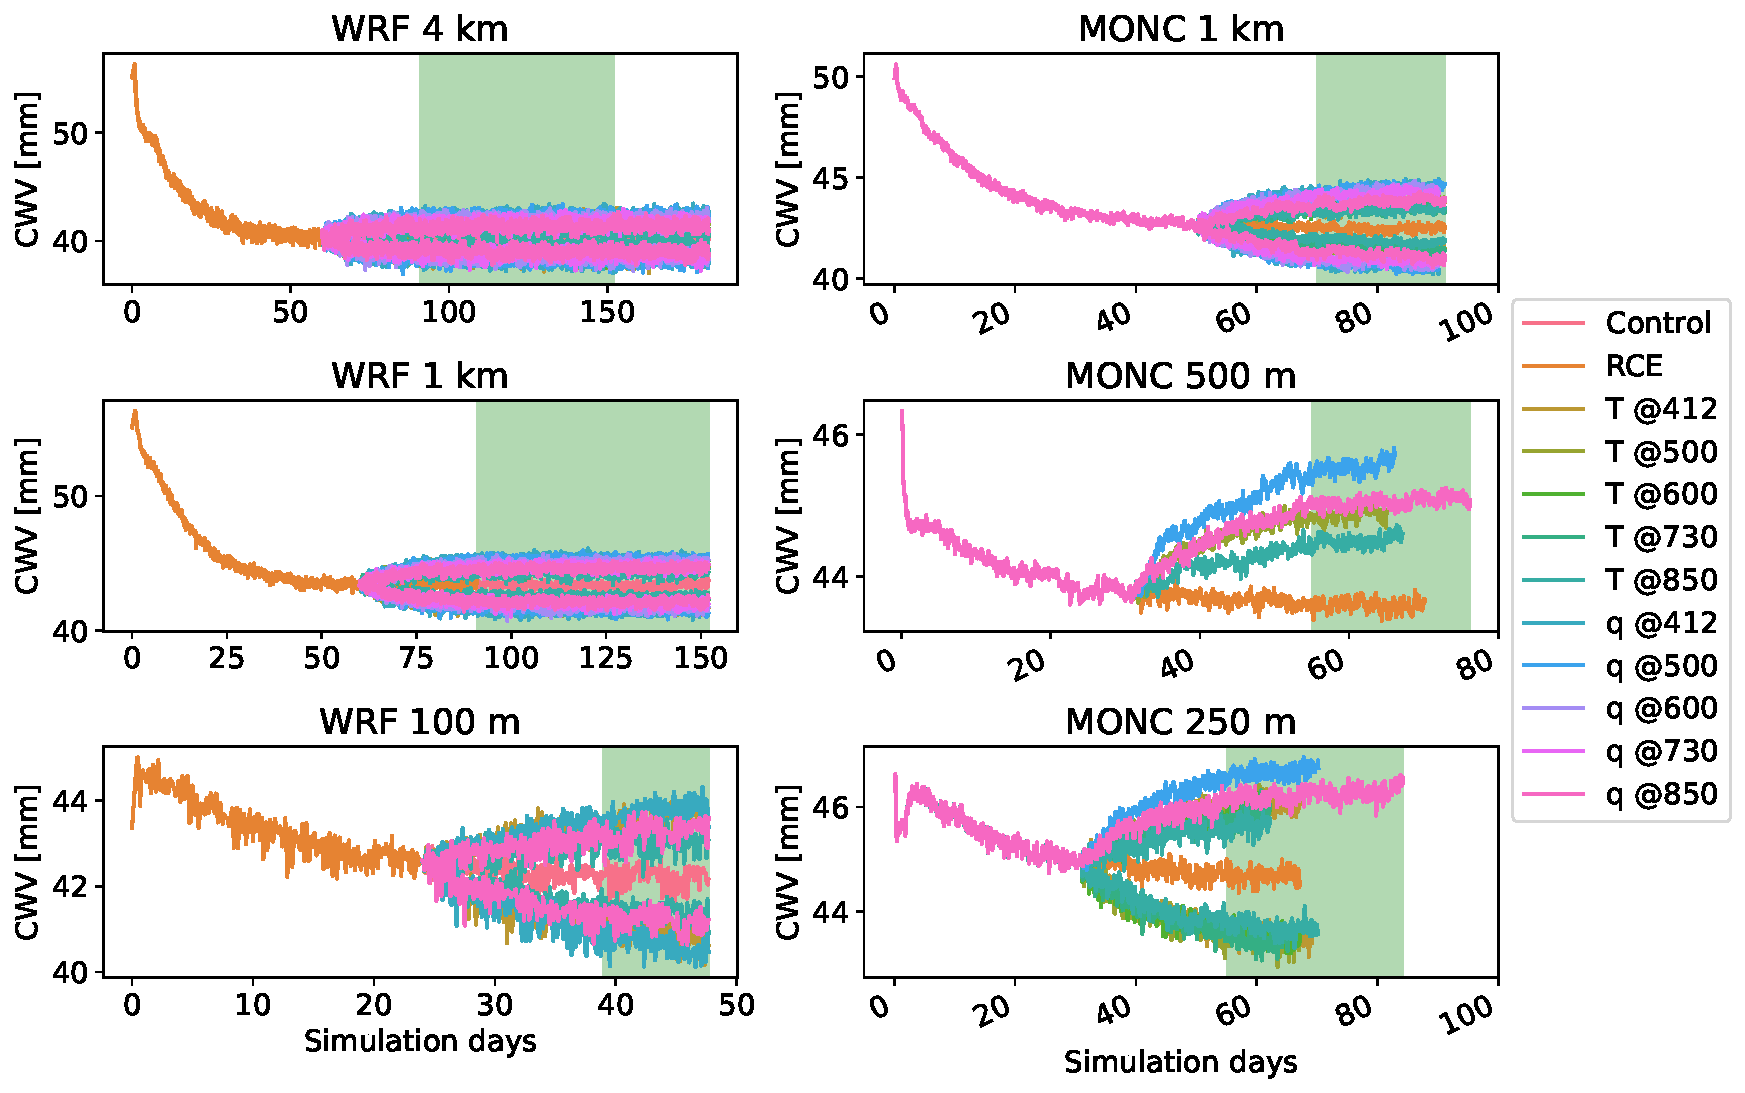
\includegraphics[width=\textwidth]{figures/runs_timeseries.pdf}
    \caption{Time series of water content (spatial mean column water vapor, CWV)
    by grid spacing in WRF and MONC. RCE runs were performed until the columnar
    water content stabilized. At this point the perturbations were introduced,
    and the model was run until all perturbed runs had also reached equilibrium.
    The parts of the time axes highlighted in green show the ``RCE region'' over
    which mean profiles were calculated for comparison. For the MONC runs, the
    highlighted region shows the maximum range of RCE regions, since RCE regions
    were defined as the last 20 days in each simulation for 1 km runs and the
    last 10 days in each simulation for the 500 m and 250 m runs. To reduce the
    number of colors required, positive and negative perturbations use the same
    color.}
    \label{fig:rce_pw}
\end{figure}

\begin{figure}[h]
    \noindent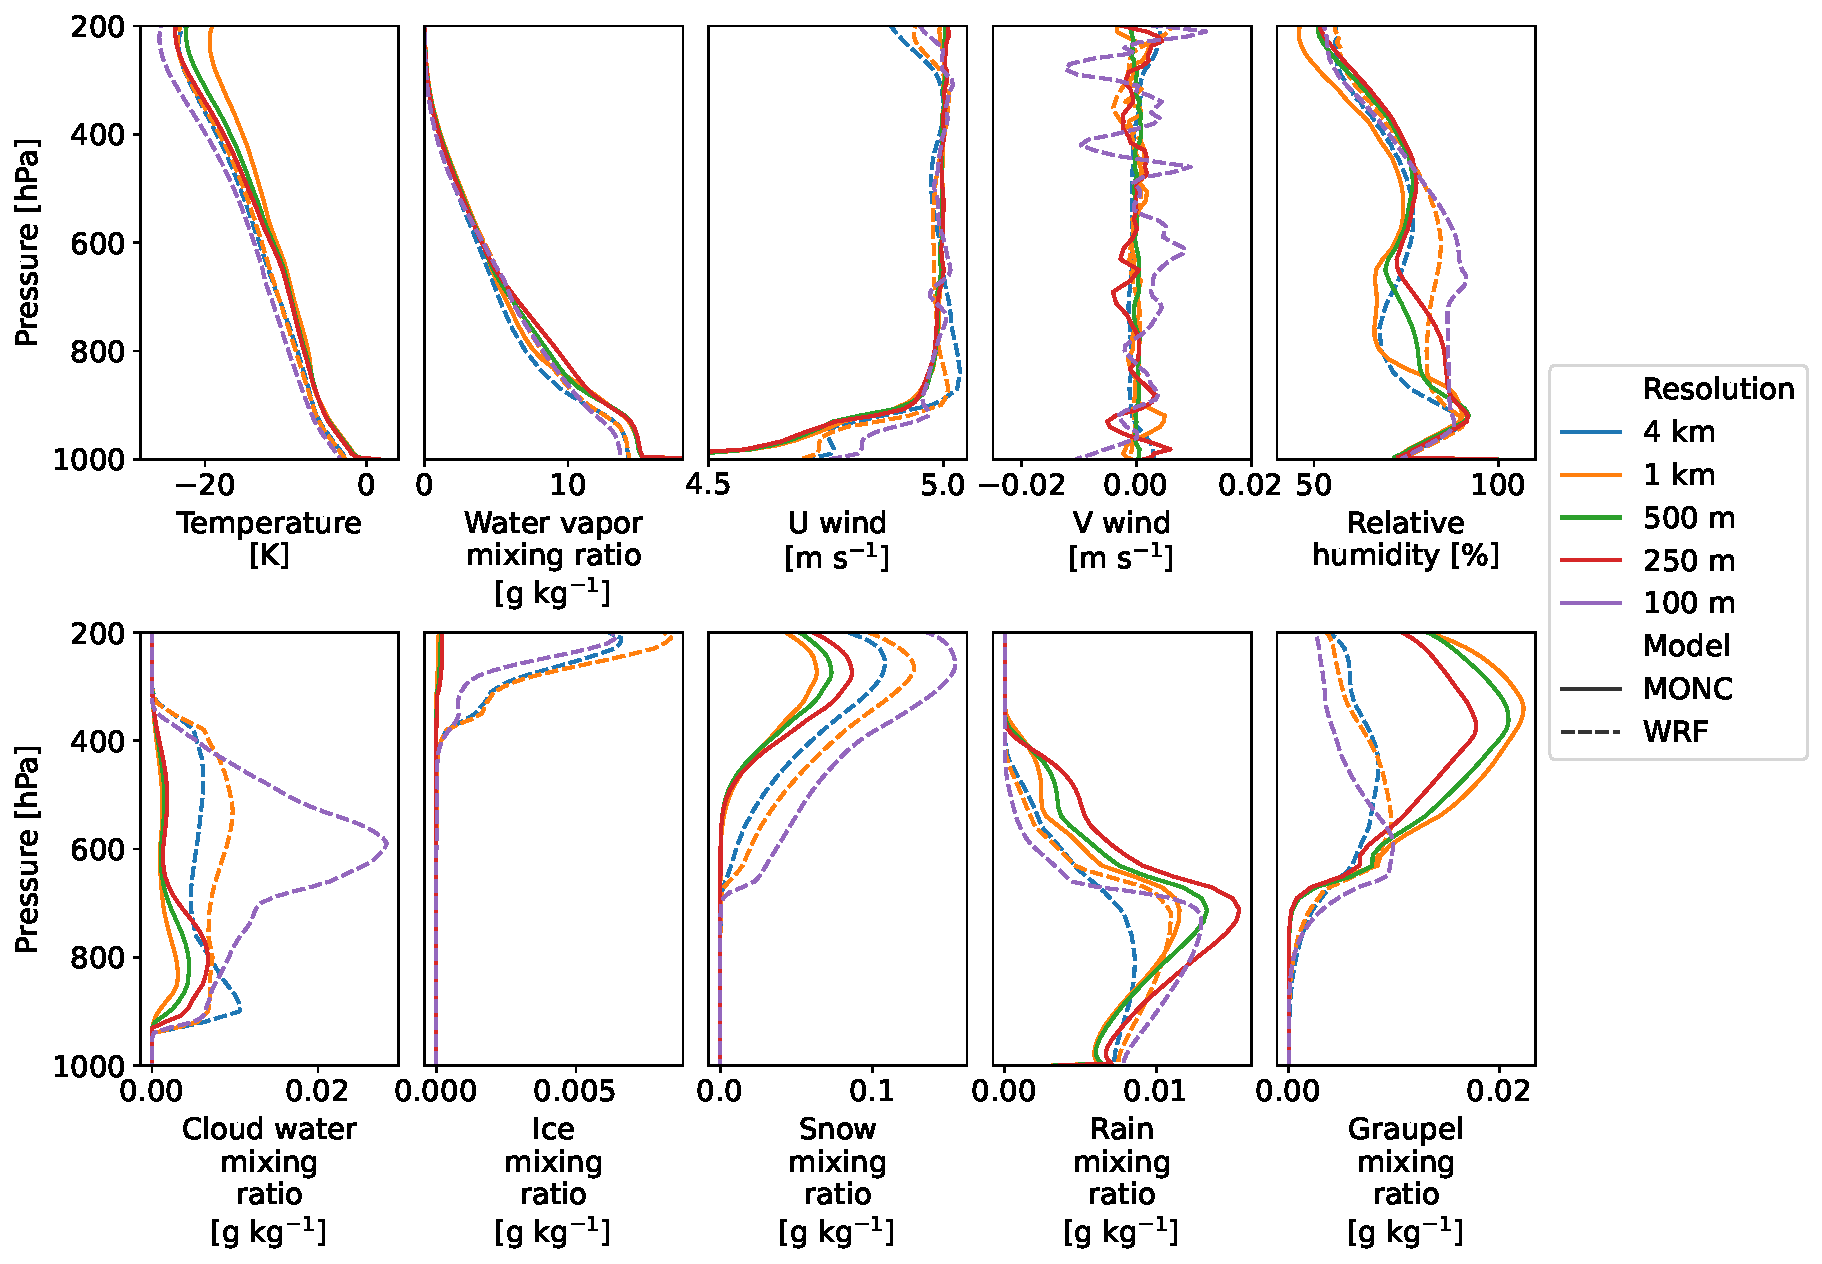
\includegraphics[width=\textwidth]{figures/rce_profiles}
    \caption{Mean profiles for selected variables in the control runs' RCE
    periods, by grid spacing. All plots stop at 200 hPa, such that a thin cirrus
    layer that formed at the tropopause in the MONC simulations is not shown
    here. Temperatures are shown as anomalies from a reference moist
    pseudo-adiabat calculated using a surface temperature of 300 K.}
    \label{fig:rce_profiles}
\end{figure}

Hydrometeor profiles were sensitive to resolution and model (Figure
\ref{fig:rce_profiles}, bottom row). In general WRF produced more cloud liquid
water and snow, and less graupel, near and above the freezing level, and less
graupel. For the WRF runs, finer resolution resulted in substantially more cloud
water and snow mass above 500 hPa or so. MONC runs were marginally less
resolution-sensitive, but the character of the changes was broadly the same as
in WRF: the cloud water changes in MONC went in the same direction as WRF but
were located mostly below $\sim$500 hPa while the snow changes in MONC were much
smaller than in WRF. It is uncertain whether these microphysical changes are
simply a consequence of mean moisture changes or whether they reflect the impact
of cloud turbulence differences.

\subsection{Convective Organization}

We tested for convective organization, to check whether any of the between-model
or between-resolution differences may be due to some setups developing
organization. To do so, we examined the spatial variance of precipitable water
scaled by its spatial mean (not shown) for both models, and for MONC we also
examined the ``subsidence fraction'', the fractional area of the domain where
the vertically integrated mass-weighted vertical wind is negative (not shown).
These metrics showed no evidence of meaningful organization, which is expected
because we used fixed radiation everywhere without contrasting radiative cooling
profiles in moist and dry regions \cite{Muller_GRL_2015}.

\subsection{Responses to Heating (Temperature) Perturbations}

The responses to heating at 415 hPa and 850 hPa are shown in Figures
\ref{fig:tpert_412} and \ref{fig:tpert_850}, respectively, with results for
perturbations at other levels (500, 600, and 730 hPa) shown in the appendix
(Figures \ref{fig:tpert_500}, \ref{fig:tpert_600}, and \ref{fig:tpert_730}). All
responses to these perturbations are much smaller than the spread in the mean
profiles with resolution (Figure \ref{fig:rce_profiles}). WRF and MONC produced
responses of similar amplitude. Most of the experiments show approximately
linear behavior, with similar responses per unit forcing regardless of forcing
sign. The strongest nonlinearity is found in the WRF hydrometeor responses at
100 m grid spacing, but this is probably attributable to noise given the shorter
duration and high variability of responses in this experiment.

\begin{figure}[pth]
    \noindent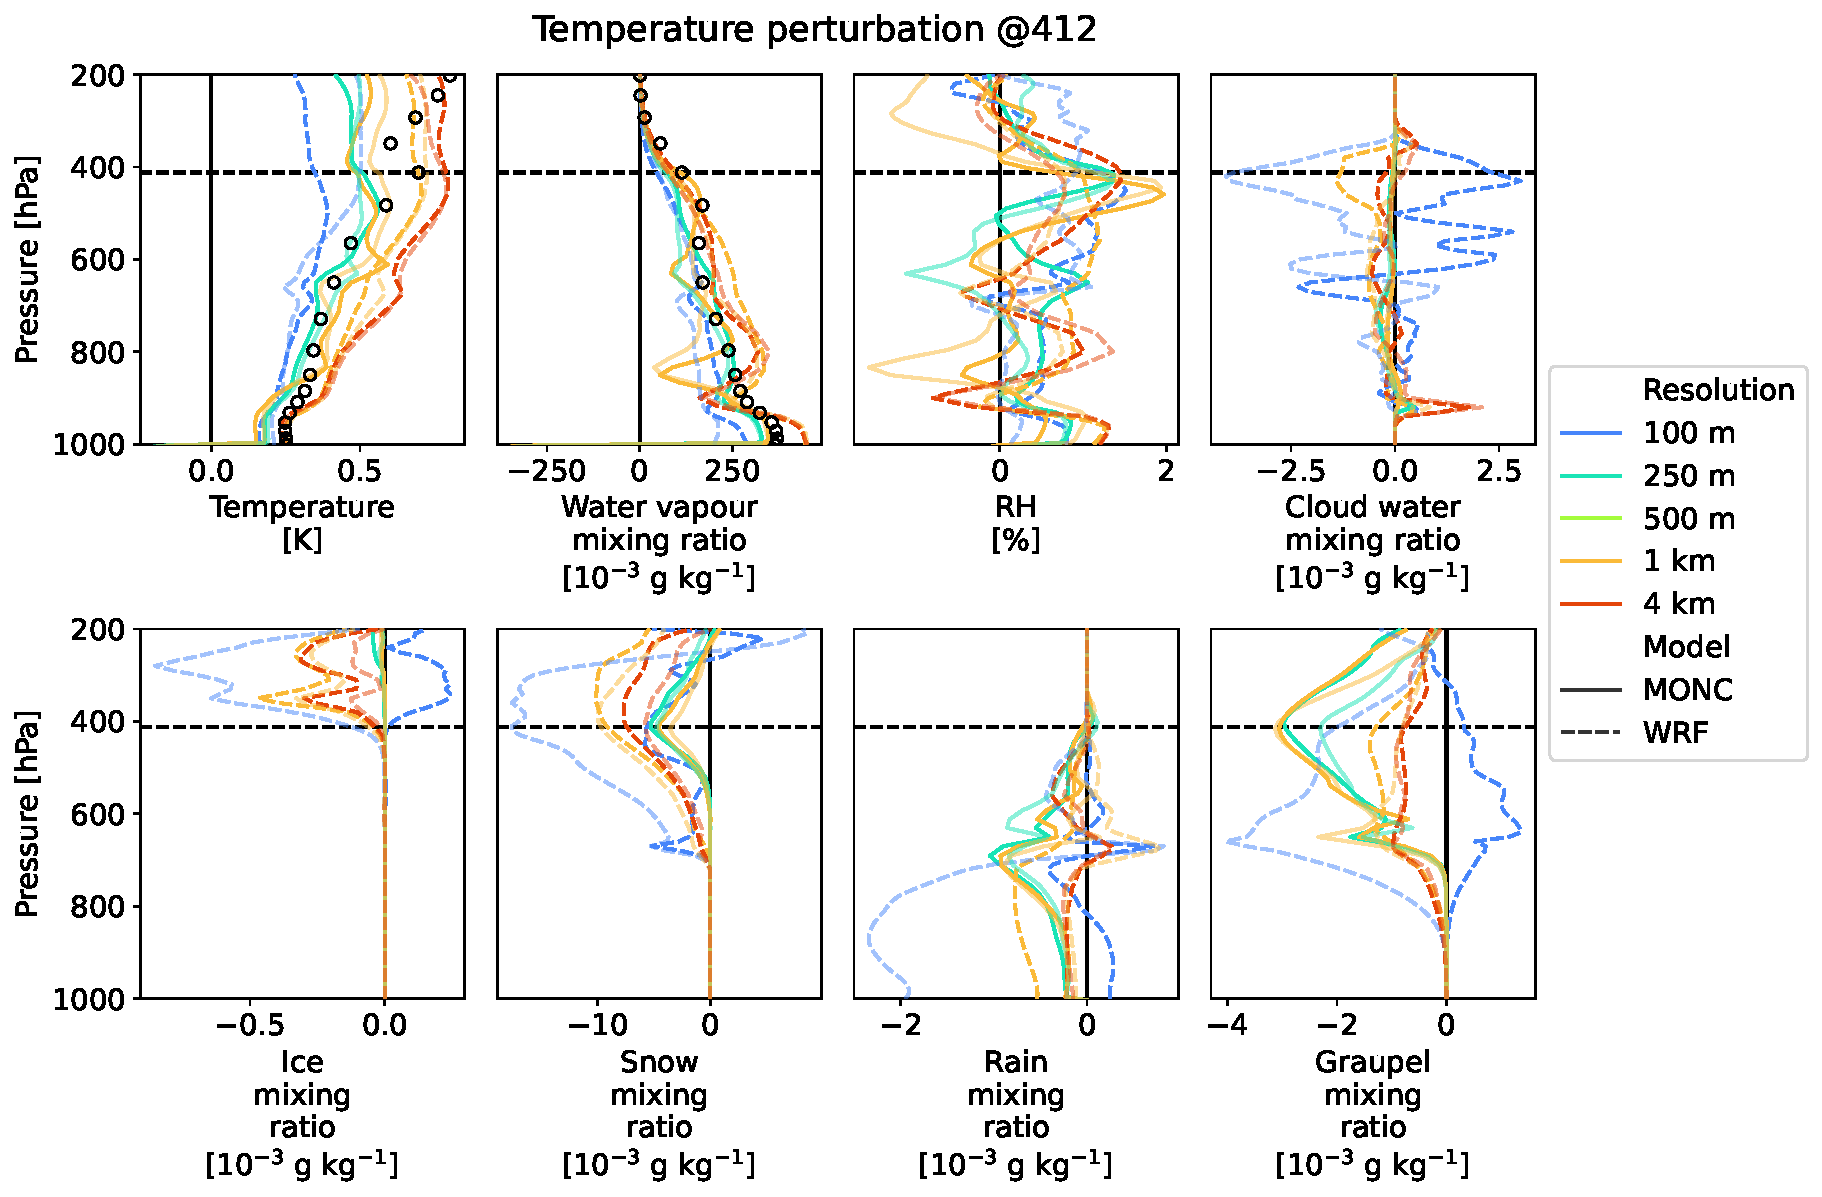
\includegraphics[width=\textwidth]{figures/pert_diffs_T_0.5_@412}
    \caption{Differences in model values by pressure, after a perturbation
    forcing of amplitude 0.5 K was introduced in temperature at 412 hPa (415 hPa
    for MONC). The solid vertical black line shows zero difference. The dashed
    horizontal line shows the approximate level of maximum perturbation.
    Responses to positive perturbations are shown with opaque lines, while
    responses to negative perturbations are shown with semi-transparent lines.
    Responses to negative perturbations have been multiplied by $-1$, so they
    overlay responses to positive perturbations if the positive and negative
    responses are symmetrical. Black circles show the responses to the same
    perturbation recorded by K10.}
    \label{fig:tpert_412}
\end{figure}

\begin{figure}[pth]
    \noindent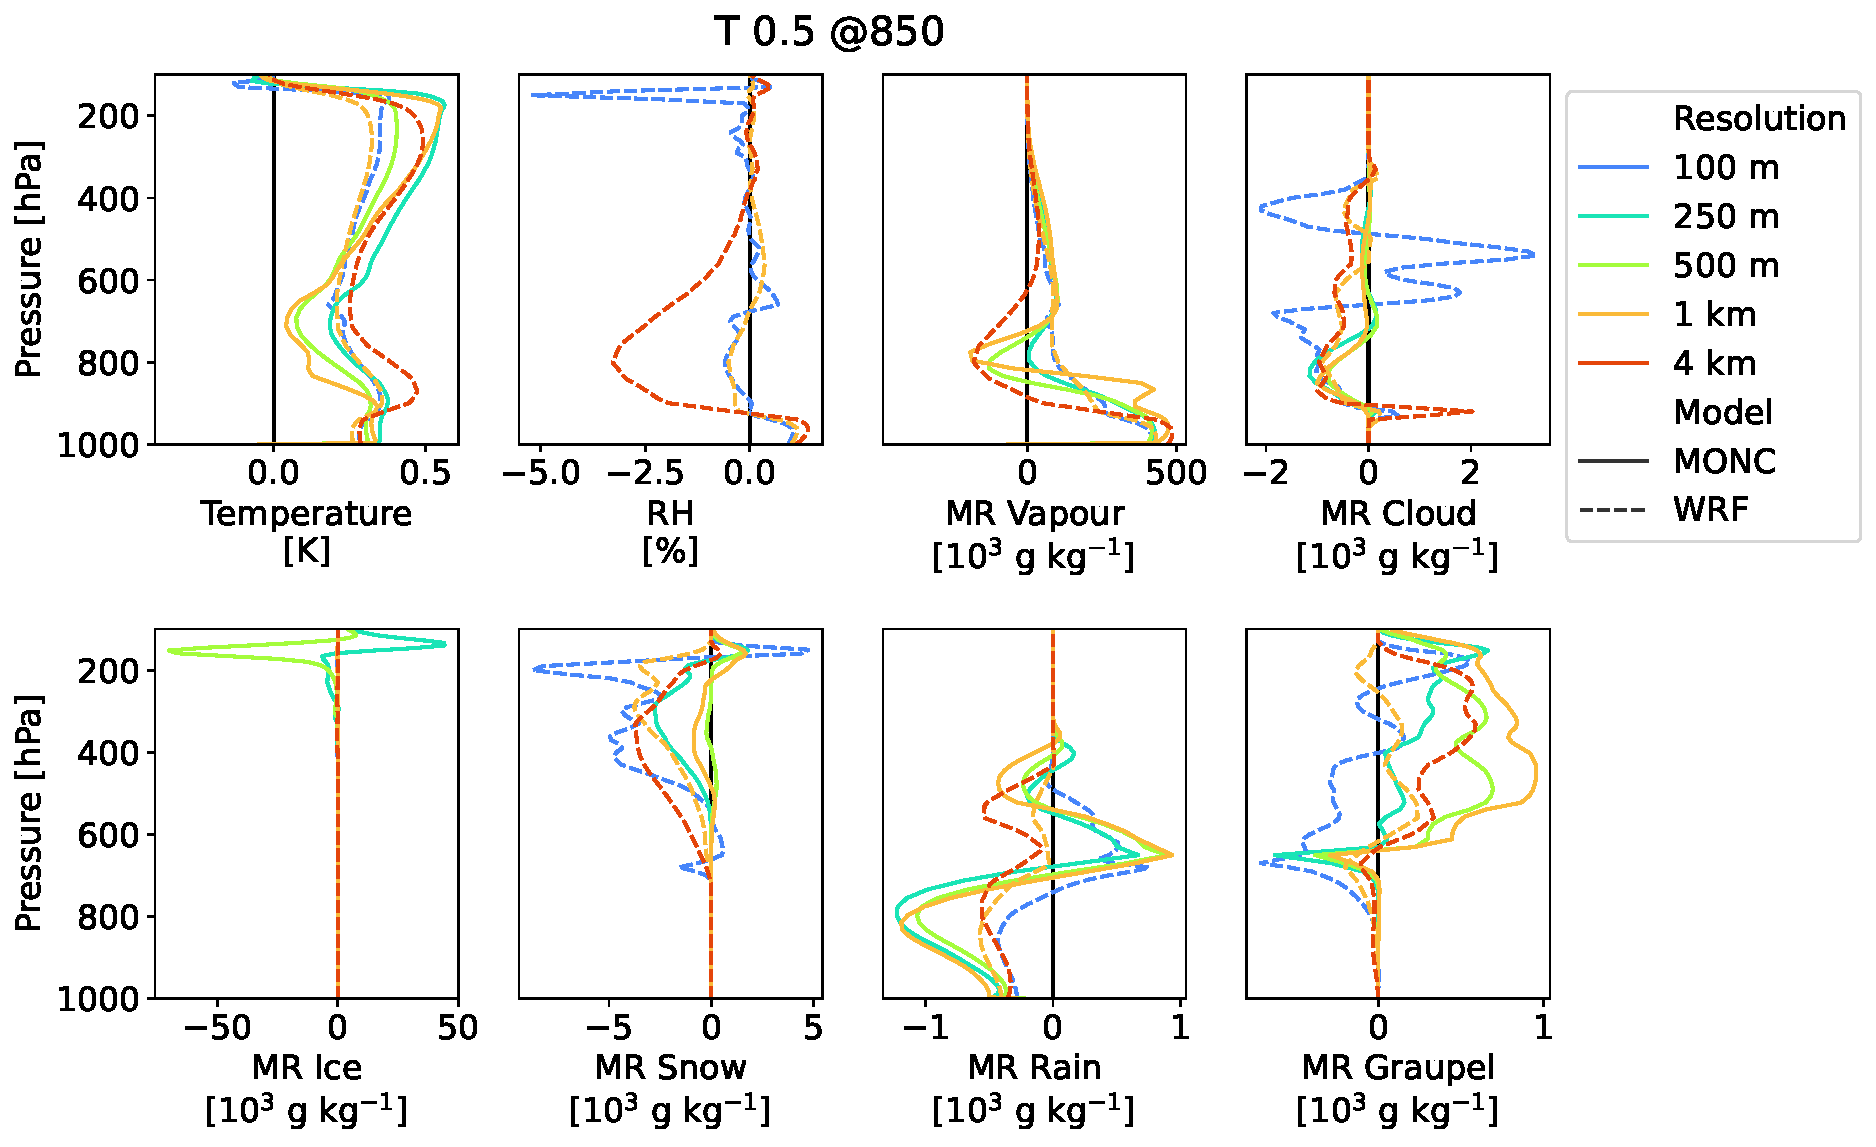
\includegraphics[width=\textwidth]{figures/pert_diffs_T_0.5_@850}
    \caption{As in Figure \ref{fig:tpert_412}, but for a temperature
    perturbation at 850 hPa.}
    \label{fig:tpert_850}
\end{figure}

\subsubsection{Temperature Responses to Heating}

Temperature responses tend to increase with height from the surface to a maximum
just below the perturbation level, then decrease around the perturbation level
before once more increasing at greater heights. This "dog leg" structure is most
apparent in the responses to perturbations in the middle levels (500, 600, 730
hPa), but not 850 hPa, and is often more marked in MONC than in WRF which gives
a smoother temperature response in the vertical. The sub-km-resolution MONC runs
produce smoother responses than the 1-km ones. The general character of this
response was already noted by K10 and H21 who explain that the trend with height
is expected from a warming pseudoadiabat, while the "dog leg" is consistent with
stabilization of the atmosphere near the heated level locally inhibiting upward
heat transport. Boundary-layer and upper-tropospheric responses differ somewhat
between the simulations, with WRF warming more than MONC from 415-hPa heating
but less from 850-hPa heating, and lower-resolution WRF showing strong
stabilization near 900 hPa for both heatings.

\subsubsection{Moisture Responses to Heating}

Heating induces an increase in water vapor mixing ratio at the perturbation
level, which increases roughly linearly (with some variation depending on model)
to the surface. This response is again smoother from WRF than from MONC. Heating
at 415 and 850 hPa produces the strongest differences among the various runs. At
coarser resolutions (WRF at 4 km grid spacing and MONC at 1 km and 500 m),
850-hPa heating can reduce the humidity at and just above the perturbation
level; With WRF, this response becomes an increase at finer resolution, while
with MONC it decreases to near zero by 250 m. For the temperature perturbation
at 850 hPa, moistening in the boundary layer reduces for finer resolutions in
WRF, and to a lesser extent for MONC. 

A temperature perturbation at 415 hPa (or down to 600 hPa, see appendix)
produces a minimum in the humidity increase in the WRF runs at around 900 hPa.
In MONC there is a similarly pronounced minimum, a little higher at about 850
hPa. This feature becomes less pronounced with increasing resolution in both
models and is not evident in K10; in WRF it occurs together with an enhanced
moisture increase near the surface at 1 and 4 km. There is often a small minimum
in the humidity increase around or at the perturbation level, particularly for
perturbations applied at lower levels (at higher levels a second minimum tends
to appear below the perturbation). For heating at 730 hPa (Figure
\ref{fig:qpert_730}) in MONC the local humidity response decreases to around
zero, but does not become negative as with 850 hPa heating. The dampened
humidity increase near and above the heated level is consistent with the
stabilization mechanism noted above; the reason for exaggerated near
boundary-layer top in coarser-resolution simulations is less obvious but likely
due to poor responses of under-resolved shallow convection. All WRF and MONC
responses show a steeper gradient from 900-950 hPa than was shown by K10,
suggesting that while the relatively coarse K10 simulations were surprisingly
accurate overall they were unable to resolve structural changes to boundary
layer moisture, due perhaps to humid convective downdrafts or changes to
boundary layer mixing.

\subsubsection{Hydrometeor Responses}

The two models show responses in hydrometeor content that are broadly similar in
character, but sometimes with large differences in magnitudes and disagreement
on resolution effects. 850 hPa heating generally reduces rain water content
below \todo{SS: Does precipitation change much in these experiments (I would
think not since we impose radiative heating)?  If not, does this reduction in
mixing ratio imply an increase in drop fall speed?  I guess it could also be a
downward shift in conversion to rain.  These could happen together as a result
of higher mixing ratios in the BL, if drop number stays the same.} the freezing
level; MONC shows a stronger reduction than WRF below the freezing level, but an
increase around the freezing level not seen in WRF. Except for an upward spike
around 900 hPa in some runs, cloud liquid water also decreases. There is also
some reduction in snow and increase in graupel at upper levels but to a highly
variable degree. Graupel and temperature changes in the upper troposphere seem
to correlate fairly well across the simulations at both heating levels, which
may indicate that the variability in freezing processes helps cause different
temperature responses. As the perturbation level increases in the WRF runs, the
graupel response flips sign, while all other changes are qualitatively not that
different. The two models showed a broadly similar character of microphysical
responses to temperature perturbations, but there were sometimes different
amplitudes of responses which are presumably attributable to differences in
microphysics schemes. The models also did not agree on how responses change with
resolution.

\subsection{Responses to Moistening (Humidity) Perturbations}

The responses to moistening at 415 and 850 hPa are shown in Figures
\ref{fig:qpert_412} and \ref{fig:qpert_850}, respectively, while those for 500,
600, and 730 hPa are shown in Figures \ref{fig:qpert_500}, \ref{fig:qpert_600},
and \ref{fig:qpert_730} respectively. Several elements of these results are
similar to those for heating: moisture and hydrometeor responses are again
smaller than the spread in mean profiles due to resolution. WRF and MONC
produced responses of similar amplitude, except for cloud liquid water and ice
where the changes in MONC were much smaller; and nonlinearities are significant
for some responses, with MONC showing more nonlinearity in thermodynamic
responses than WRF except for the (shorter) 100-m WRF runs. MONC relative
humidity seems to be prone to non-linear responses. Similar to the responses to
the temperature perturbations, the strongest apparent nonlinearity after
moisture perturbations is in the hydrometeor and relative humidity fields, and
there was a large range in responses (Figures \ref{fig:var_q_412} and
\ref{fig:var_q_850}).

\begin{figure}[pth]
    \noindent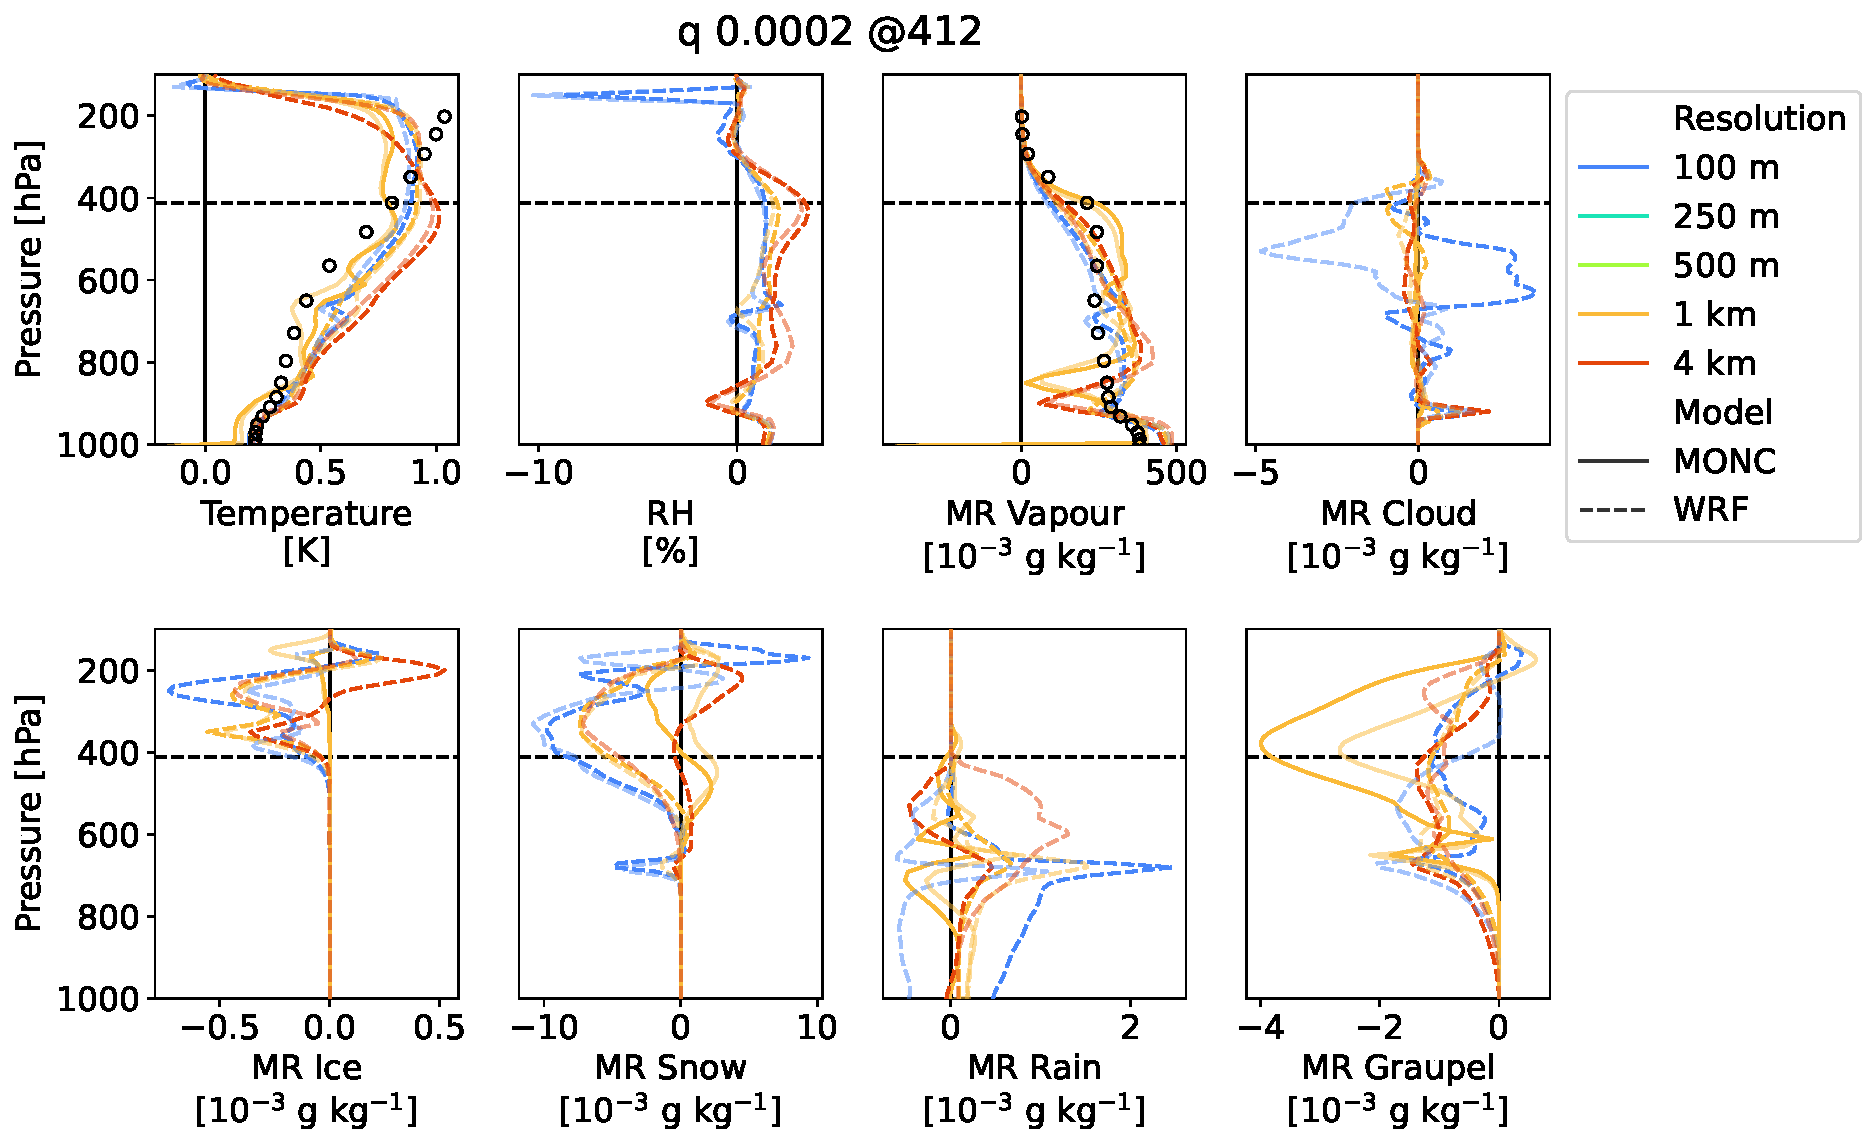
\includegraphics[width=\textwidth]{figures/pert_diffs_q_0.0002_@412}
    \caption{As for Figure \ref{fig:tpert_412}, but for differences in model
    values by pressure, after a perturbation forcing of amplitude 0.2 g
    kg$^{-1}$ was introduced in the water vapor mixing ratio tendency field at
    412 hPa (415 hPa for MONC).}
    \label{fig:qpert_412}
\end{figure}

\begin{figure}[pth]
    \noindent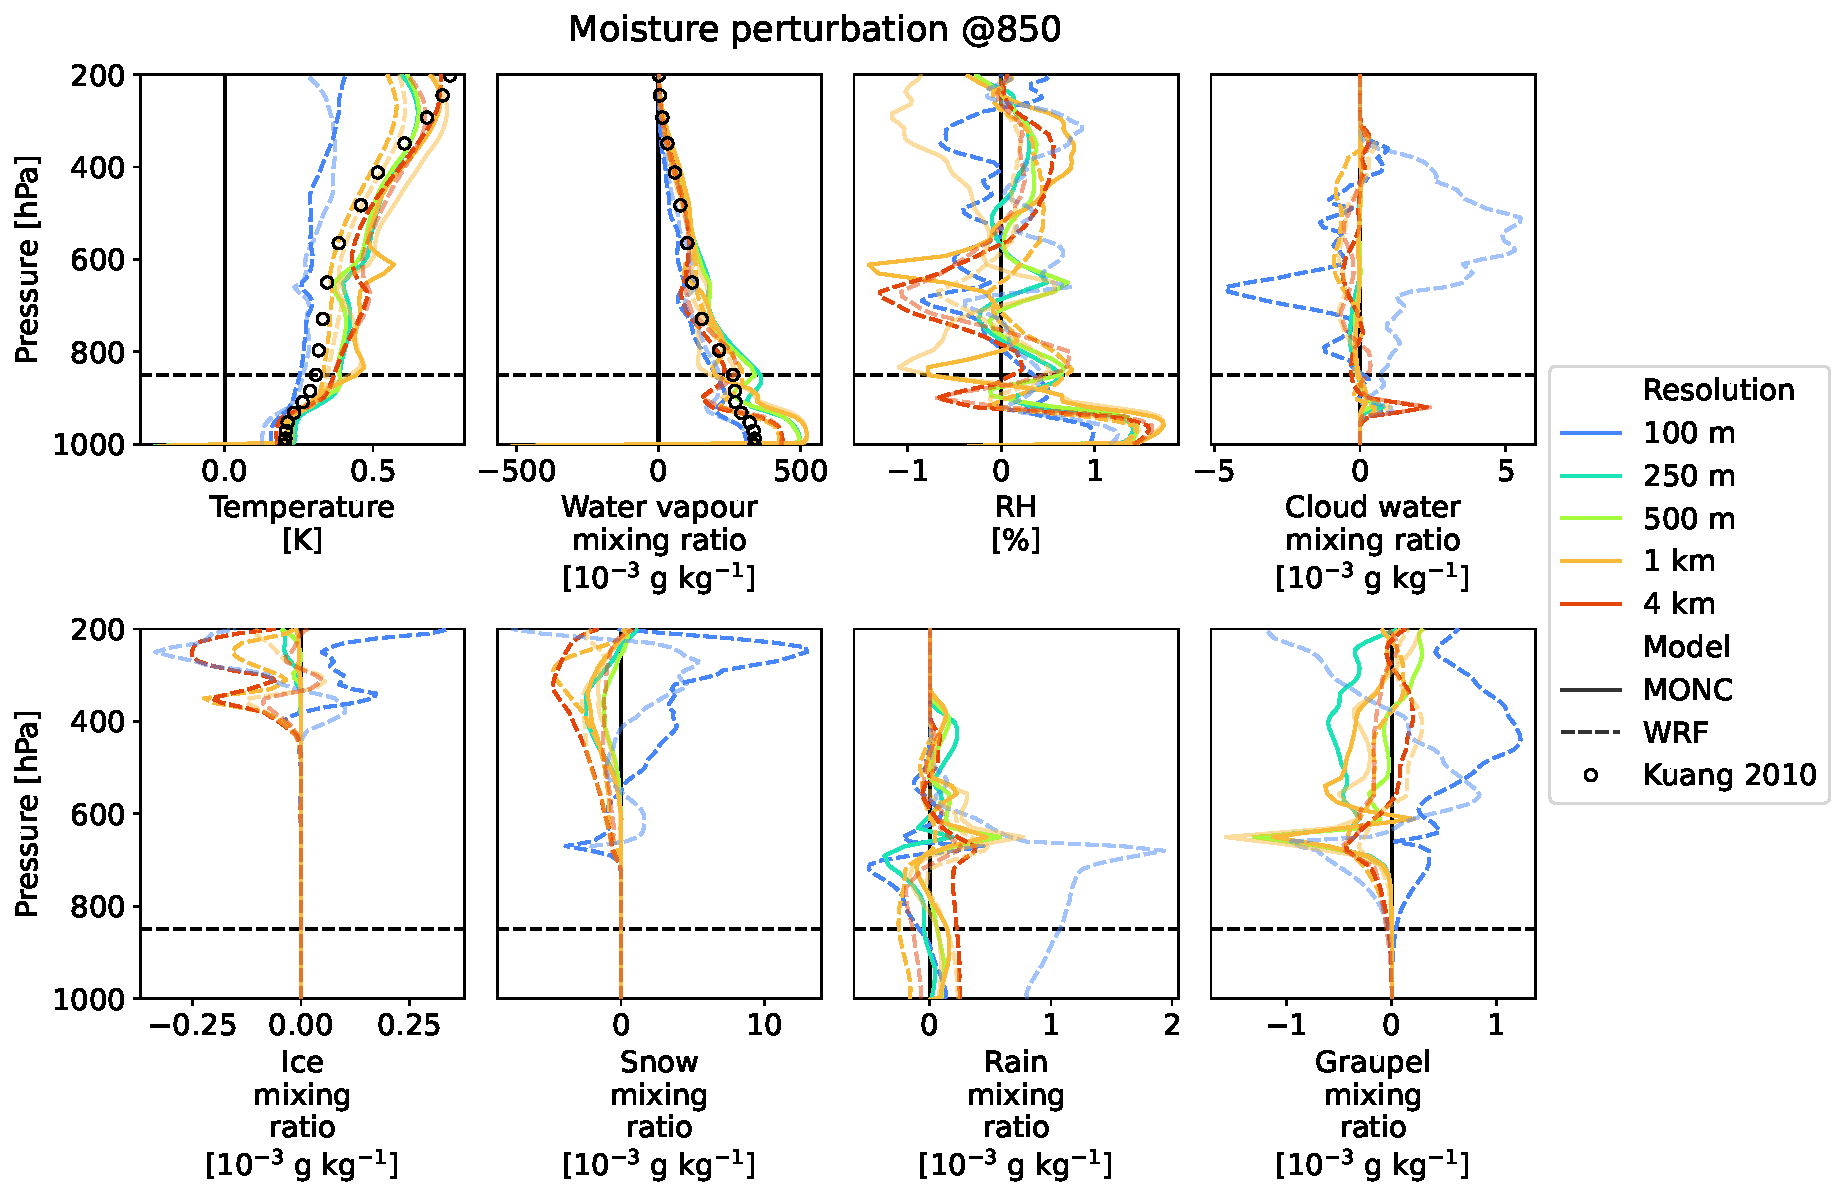
\includegraphics[width=\textwidth]{figures/pert_diffs_q_0.0002_@850}
    \caption{As in Figure \ref{fig:qpert_412}, but for a water vapor mixing
    ratio perturbation at 850 hPa.}
    \label{fig:qpert_850}
\end{figure}

\subsubsection{Temperature Responses to Moistening}

Temperature increases again increase with height as expected from a moist
adiabat (though without the "dog leg" induced by heating).  Temperature
increases in the boundary layer are very consistent between resolutions in WRF.
Those in the free troposphere are somewhat more consistent from moistening than
seen earlier for heating perturbations, but do strengthen with increasing grid
size, especially for moistening at 412 hPa. MONC responses show weak
resolution-dependence between about 600 and 850 hPa, but elsewhere show some
sensitivity in the opposite direction to that in WRF. The boundary-layer
temperature increases are more consistent between WRF and MONC than for heating.
The free-tropospheric increases are stronger in MONC than WRF for a low-level
moisture perturbation and weaker for an upper-level moisture perturbation. It is
notable that, for instance, the temperature response above 300 hPa to a moisture
perturbation at 850 hPa appears to show greater variability than the
corresponding spread observed in the SCMs in H21.

\subsubsection{Humidity Responses to Moistening}

Results show similar increases in water vapor mixing ratio as seen with heating
except that, as expected, relative humidity increases near the moistening level.
The humidity reductions at upper PBL levels seen above for heating perturbations
appear again here, and again decrease at finer grid spacings. Also, we again see
strong gradients in the humidity response near 925 hPa, which are smoothed out
in K10.

\subsubsection{Hydrometeor Responses to Moistening}

The hydrometeor responses to moistening share many characteristics with those
seen above for heating, with a few interesting differences.  First, graupel
decreases strongly for either lower- or upper-level moistening, showing that
low-level sources of heat and humidity affect intense convection very
differently, and the graupel responses no longer correlate with those of
upper-tropospheric temperature.  Second, responses of cloud and rain water are
more muted. These differences indicate that low-level heating, more so than
moistening, provokes important microphysical changes in deep convection (that
vary among the models here).

\section{Conclusions}
\label{sec:conclusions}

In this work we examined time-averaged responses to temperature and moisture
forcing perturbations in simulated RCE states, using two models at a range of
grid spacings including LES runs without PBL schemes enabled. The aim has been
to test the sensitivity of responses to model parameterizations and resolution.
The study builds on \citeA{Kuang_JAS_2010}, here K10, who first calculated such
responses, and other studies (in particular \citeA{Hwong_JAMES_2021}, here H21)
who used them to test convective schemes used in global models.

We sought a ``truth'' response or benchmark results against which other models
could be tested. The linear responses in our results are sensitive to model
resolution and model used, but do show a tendency to produce smoother vertical
structures and indications of convergence as grid spacing is reduced, suggesting
that model disagreement and artifacts from parameterizations or numerics are
reduced at finer resolutions. The temperature and water vapor responses tend to
be closer to the results of K10 as grid spacing becomes finer, indicating
surprising accuracy of these 2 km grid spacing calculations. However, above
$\sim$500 hPa we find a smaller mean response than in K10, while in the boundary
layer we find gradients in response within the lowest kilometer of the
atmosphere that were not shown in the early study. The question is, then, what
resolution is required to consider a response a benchmark result?

We can narrow down the grid spacing required to properly represent
convective-scale feedbacks on large scale flows by examining the sensitivity of
the feedbacks to model settings. From our results, it appears that model-based
differences between responses to perturbations do not start to disappear until
the grid spacing is below $\sim$1 km, and perhaps lower for responses in the
upper troposphere. While apparent convergence at grid spacings less than $\sim$1
km appears across our results, we note that variability across perturbations was
present and computational limitations precluded us from performing rigorous
convergence tests. Nonetheless, these convergence results do suggest that for
most models, to simulate convectively-coupled dynamics correctly will likely
require better resolution than is currently used in, for example, DYAMOND
\cite{Stevens_PEPS_2019}. Our results also suggest that, in the lower
troposphere, tangent linear responses are similar across the two LES models
tested here, implying they could make reasonable benchmark estimates of model
responses. In the upper troposphere the results diverge more and therefore the
error bars on responses in this region are larger. Responses for larger grid
spacings than $\sim$1 km diverge significantly from the LES responses.

A comparison of our findings with those of the SCM responses in H21 reveals
several observations. The variations in responses across different convective
parameterizations in H21 are generally more pronounced than the discrepancies
within our higher-resolution CRM and LES responses as well as K10. This suggests
that high-resolution model outputs can serve as a valuable benchmark for
identifying substantial deficiencies in convective parameterizations,
particularly when the latter deviate significantly from the responses observed
in these simulations. For instance, the pronounced kinks frequently observed in
the SCM responses -- especially near critical atmospheric levels such as the
freezing level and cloud base -- appear less prominent or even disappear at
finer resolutions in our results, underscoring the problematic threshold-like
behavior of convective parameterizations. However, this conclusion does not hold
uniformly throughout the entire atmospheric column: the temperature responses
show increasing spread at higher altitudes, at times exceeding those of the SCMs
in H21. 

In this study we also compared concentrations of hydrometeors and their
responses. Concentrations of snow and graupel in control runs, and responses of
these (and of rain mixing ratio) in experiments, were highly diverse and appear
likely to be responsible for some of the surprisingly large spread in upper-
troposphere temperature responses and perhaps others. The treatment (often
implicit) of microphysics within convection schemes may lack the diversity or
sensitivity exhibited here in the LES and CRM models, explaining the narrower
range of temperature responses in H21; this would imply that the true
uncertainty of some responses exceeds the spreads reported in H21.

In summary, the key conclusions of our study are as follows:

\begin{enumerate}
    \item For the two models tested here, correct simulation of
    convectively-coupled dynamics appears to require a grid spacing finer than
    $\sim$1 km.
    \item The linear responses of the two LES models tested here could
    reasonably be used as ground truth for GCM scheme testing within the mid and
    lower troposphere.
\end{enumerate}

We note that boundary-layer responses may still not be accurate without even
finer grids than used here, and that better representation of microphysics in
deep convection (graupel, for example) will be critical to further constrain the
results, especially in the upper troposphere. Future work should investigate
finer resolutions, and could attempt to determine whether the response is
dominated by the modelled convection itself, or whether it might be sensitive to
the specification of surface properties in an idealized modelling setting.

\section{Open Research}

Analysis code for this work, including modified WRF implementation code, WRF namelists, and all responses reported here in machine readible form, are provided at \todo{DOI}. \todo{Bob, what MONC config files could we include?}

% AGU requires an Availability Statement for the underlying data needed to
% understand, evaluate, and build upon the reported research at the time of peer
% review and publication.

% Authors should include an Availability Statement for the software that has a
% significant impact on the research. Details and templates are in the
% Availability Statement section of the Data and Software for Authors Guidance:
% \url{https://www.agu.org/Publish-with-AGU/Publish/Author-Resources/Data-and-Software-for-Authors#availability}

% It is important to cite individual datasets in this section and, and they must
% be included in your bibliography. Please use the type field in your bibtex file
% to specify the type of data cited. Options include [Dataset], [Software],
% [ComputationalNotebook], [Collection].
% Example:
%
%@misc{https://doi.org/10.7283/633e-1497,
%  doi = {10.7283/633E-1497},
%  url = {https://www.unavco.org/data/doi/10.7283/633E-1497},
%  author = {de Zeeuw-van Dalfsen, Elske and Sleeman, Reinoud},
%  title = {KNMI Dutch Antilles GPS Network - SAB1-St_Johns_Saba_NA P.S.},
%  publisher = {UNAVCO, Inc.},
%  year = {2019},
%  type = {dataset}
%}

\bibliography{library}

\newpage
\section*{Appendix}
\setcounter{figure}{0}
\renewcommand{\thefigure}{A\arabic{figure}}

\begin{figure}[pth]
    \noindent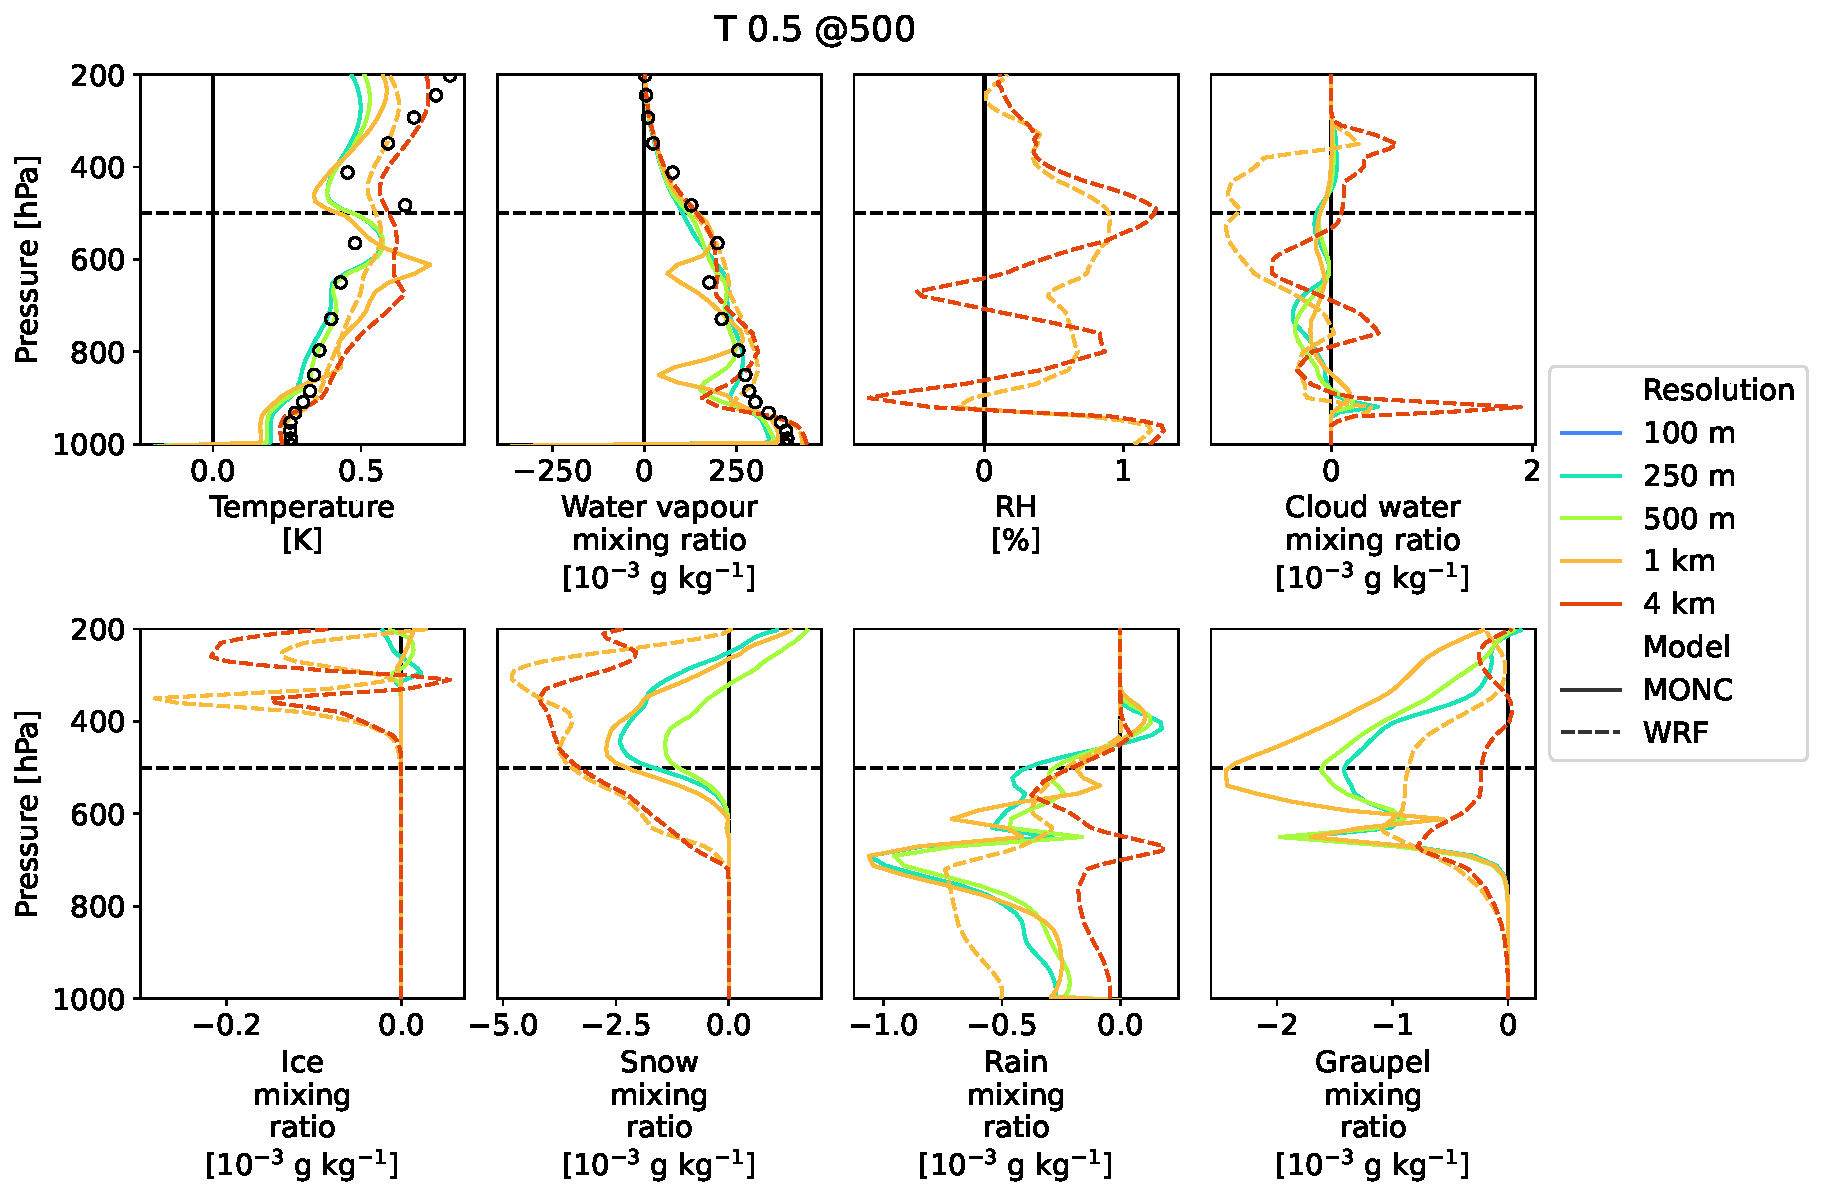
\includegraphics[width=\textwidth]{figures/pert_diffs_T_0.5_@500}
    \caption{As in Figure \ref{fig:tpert_412}, but for a temperature
    perturbation at 500 hPa, and with black circles showing the responses of K10
    to a temperature perturbation at 483 hPa.}
    \label{fig:tpert_500}
\end{figure}

\begin{figure}[pth]
    \noindent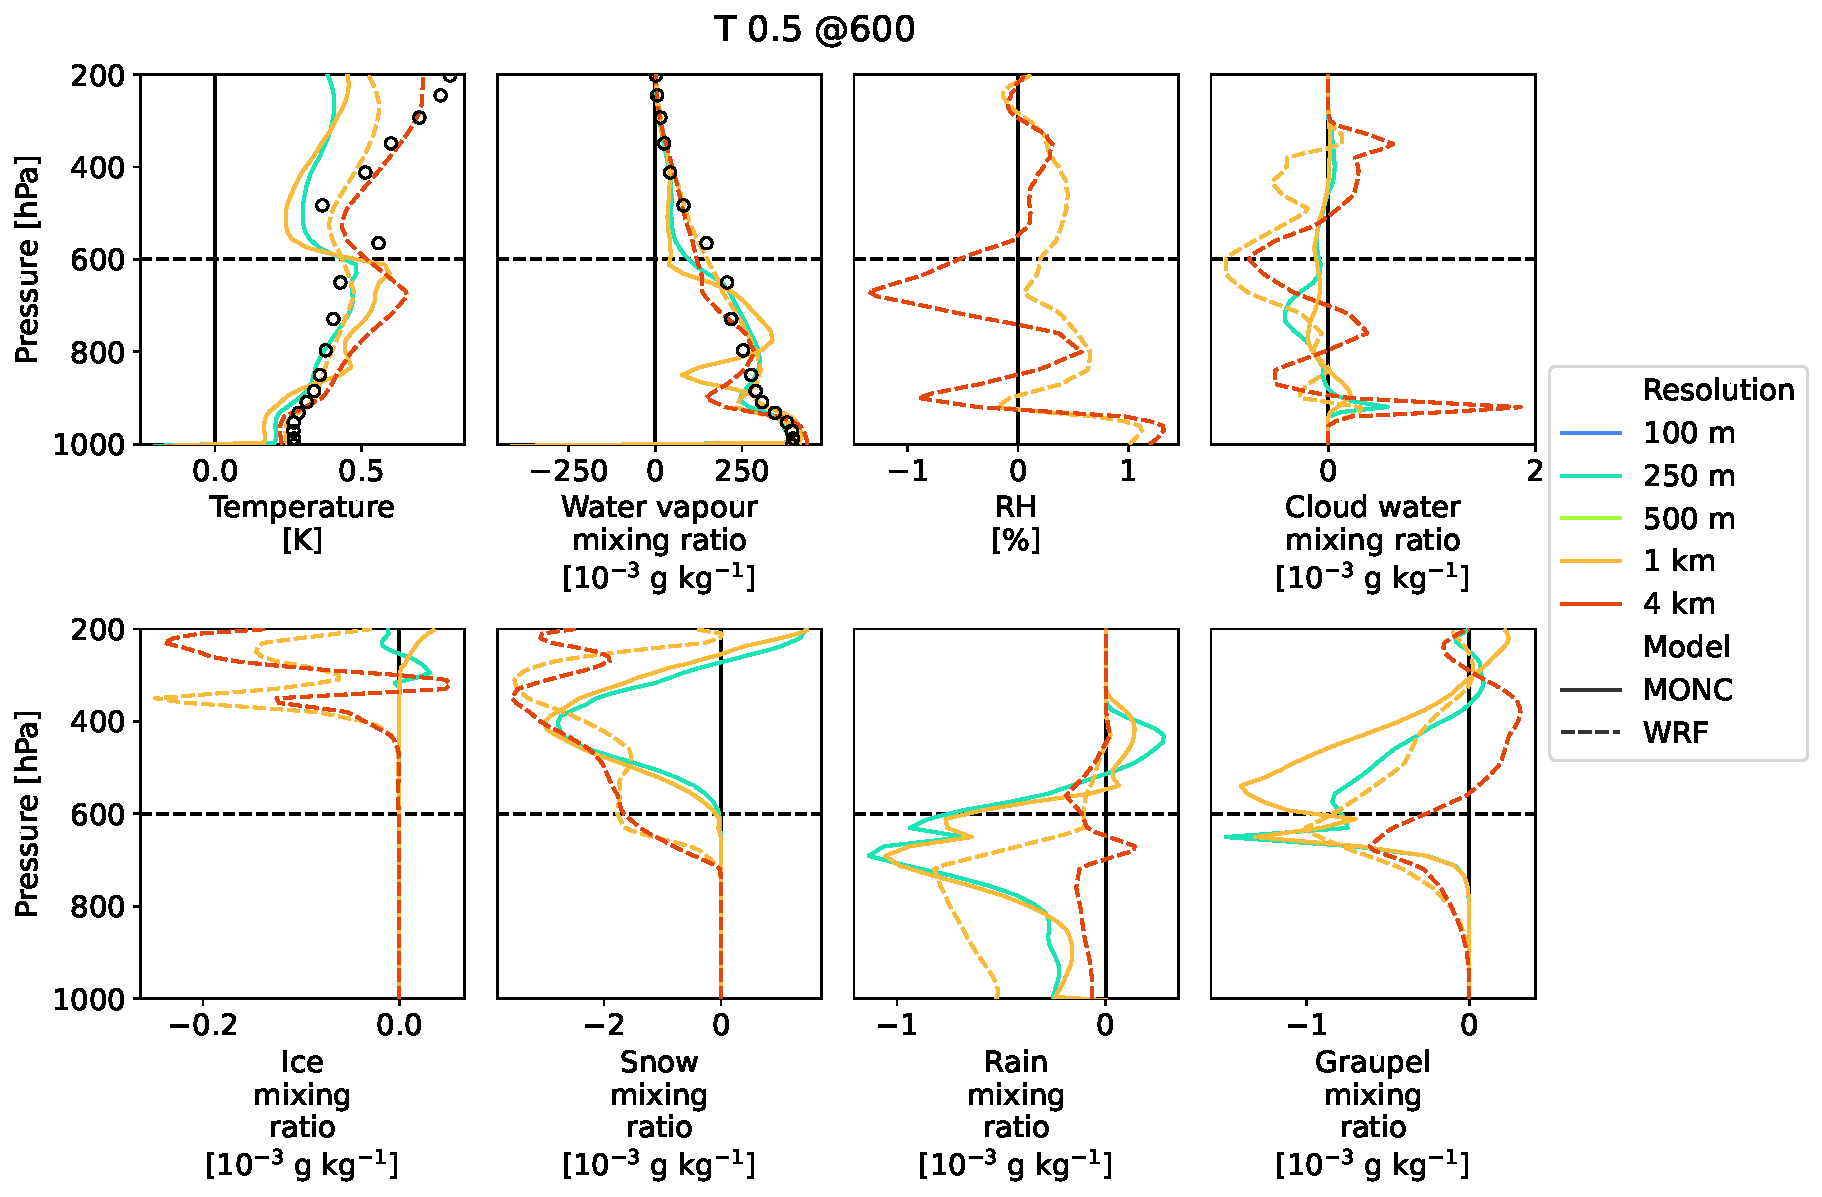
\includegraphics[width=\textwidth]{figures/pert_diffs_T_0.5_@600}
    \caption{As in Figure \ref{fig:tpert_412}, but for a temperature
    perturbation at 600 hPa, and with black circles showing the responses of K10
    to a temperature perturbation at 565 hPa.}
    \label{fig:tpert_600}
\end{figure}

\begin{figure}[pth]
    \noindent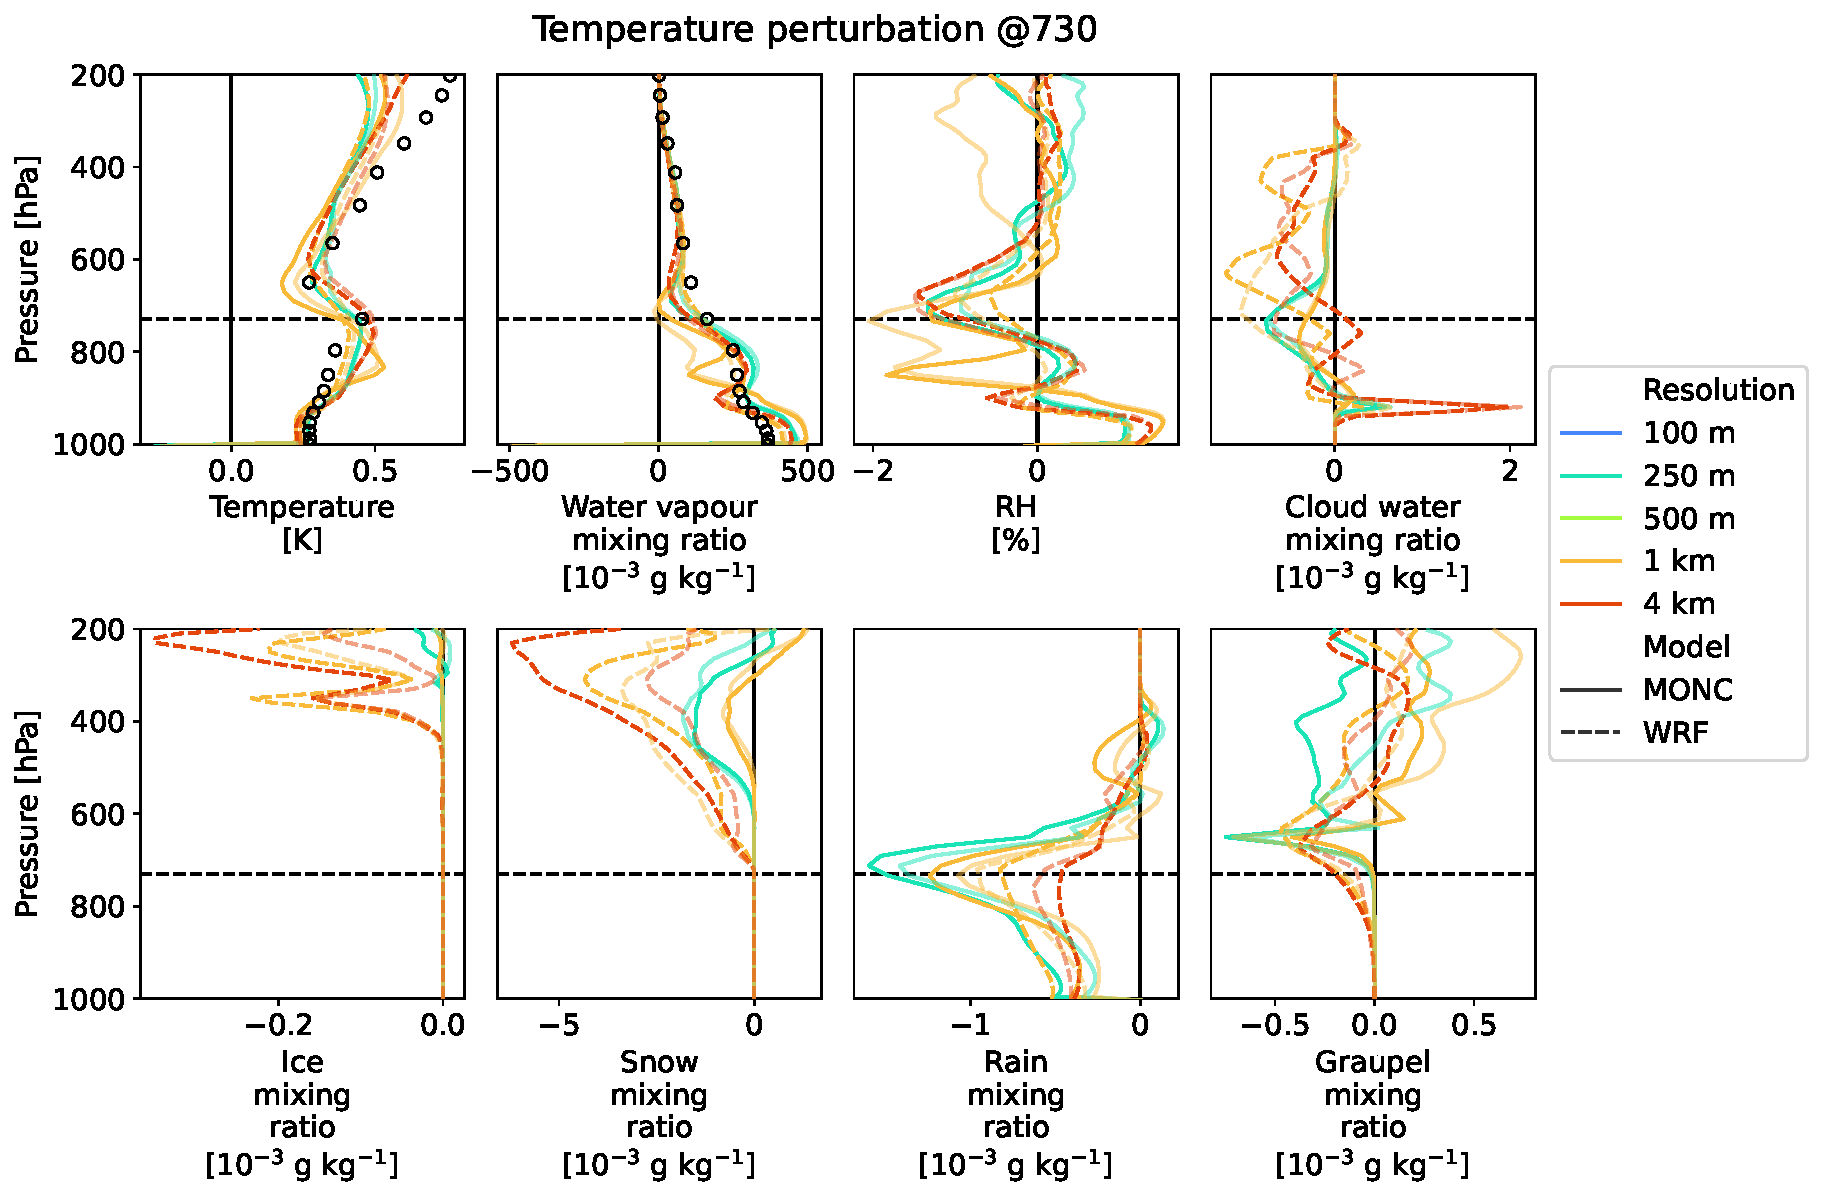
\includegraphics[width=\textwidth]{figures/pert_diffs_T_0.5_@730}
    \caption{As in Figure \ref{fig:tpert_412}, but for a temperature
    perturbation at 730 hPa, and with black circles showing the responses of K10
    to a temperature perturbation at 729 hPa.}
    \label{fig:tpert_730}
\end{figure}

\begin{figure}[pth]
    \noindent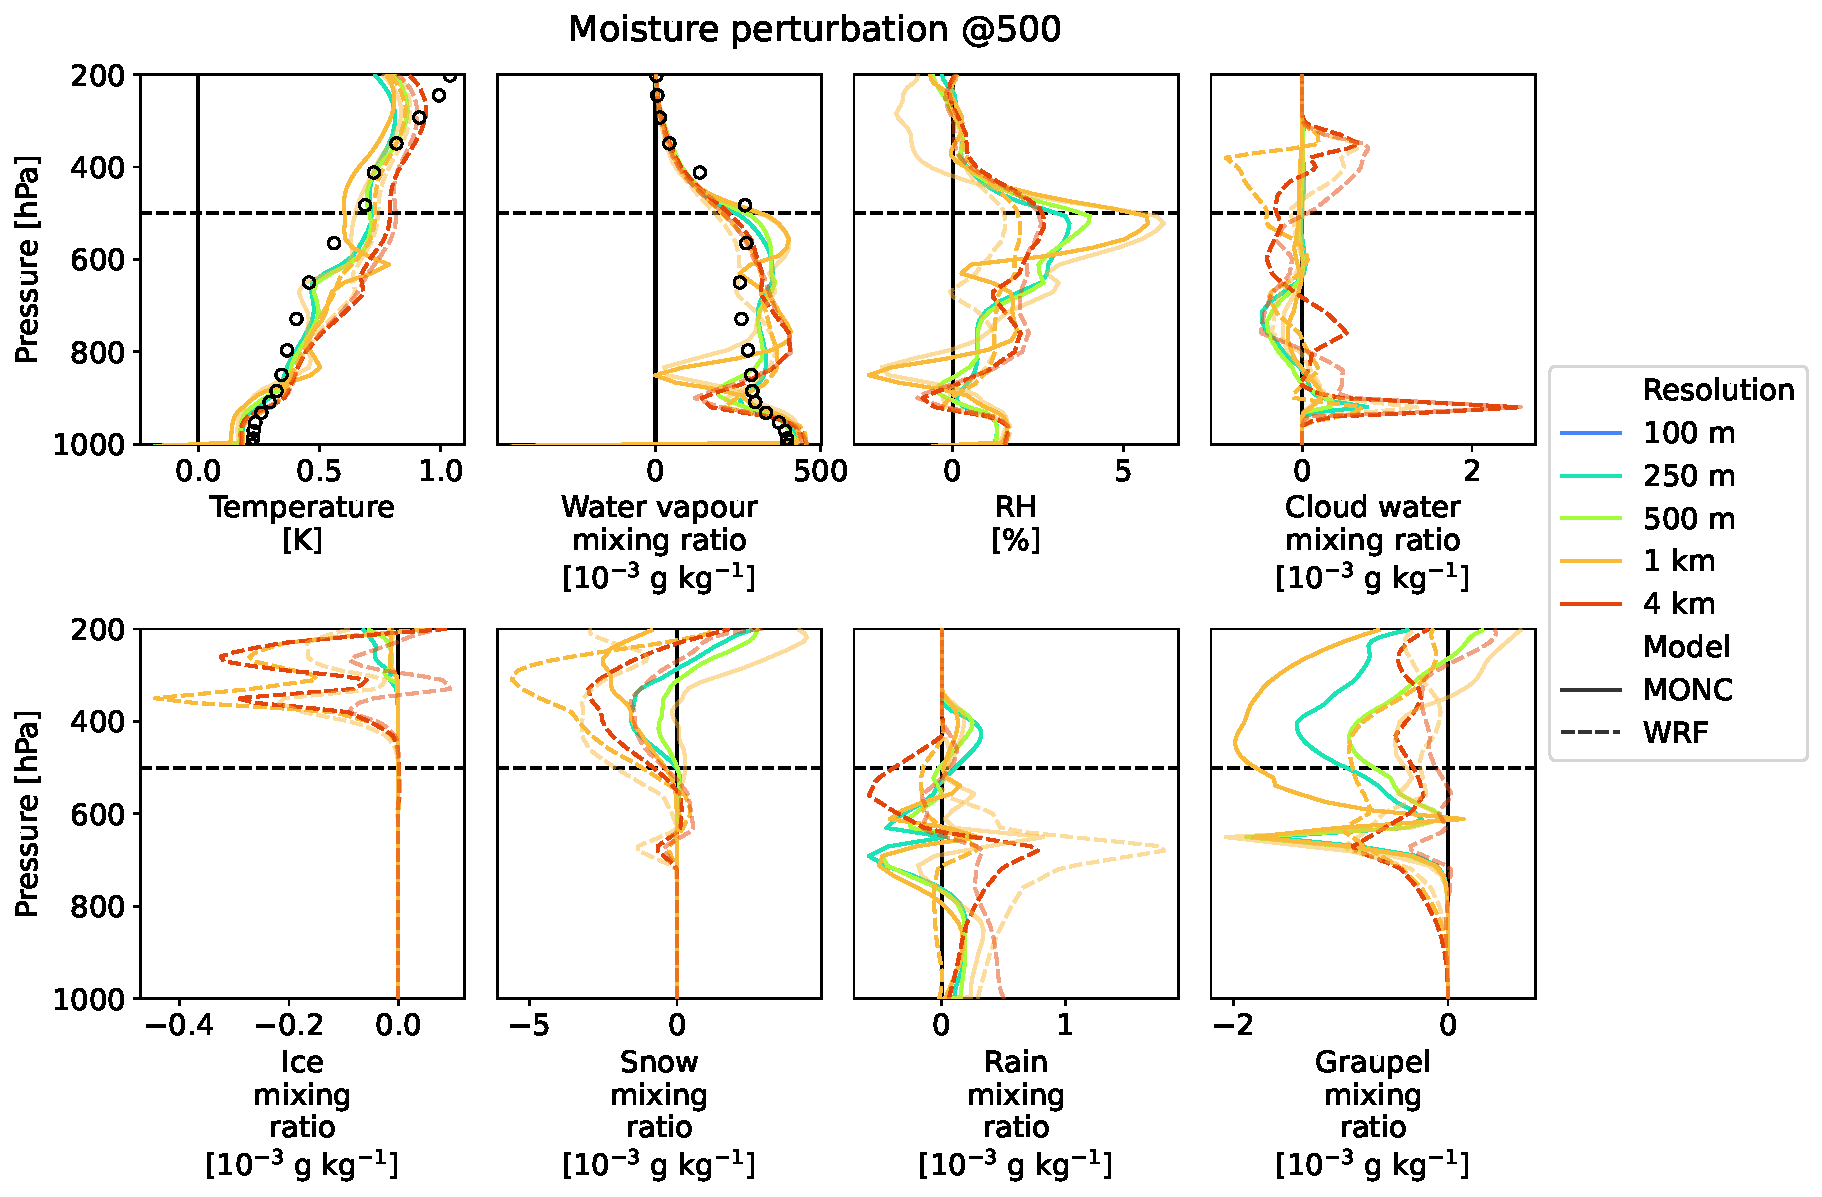
\includegraphics[width=\textwidth]{figures/pert_diffs_q_0.0002_@500}
    \caption{As in Figure \ref{fig:qpert_412}, but for a water vapor mixing
    ratio perturbation at 500 hPa, and with black circles showing the responses
    of K10 to a specific humidity perturbation at 483 hPa.}
    \label{fig:qpert_500}
\end{figure}

\begin{figure}[pth]
    \noindent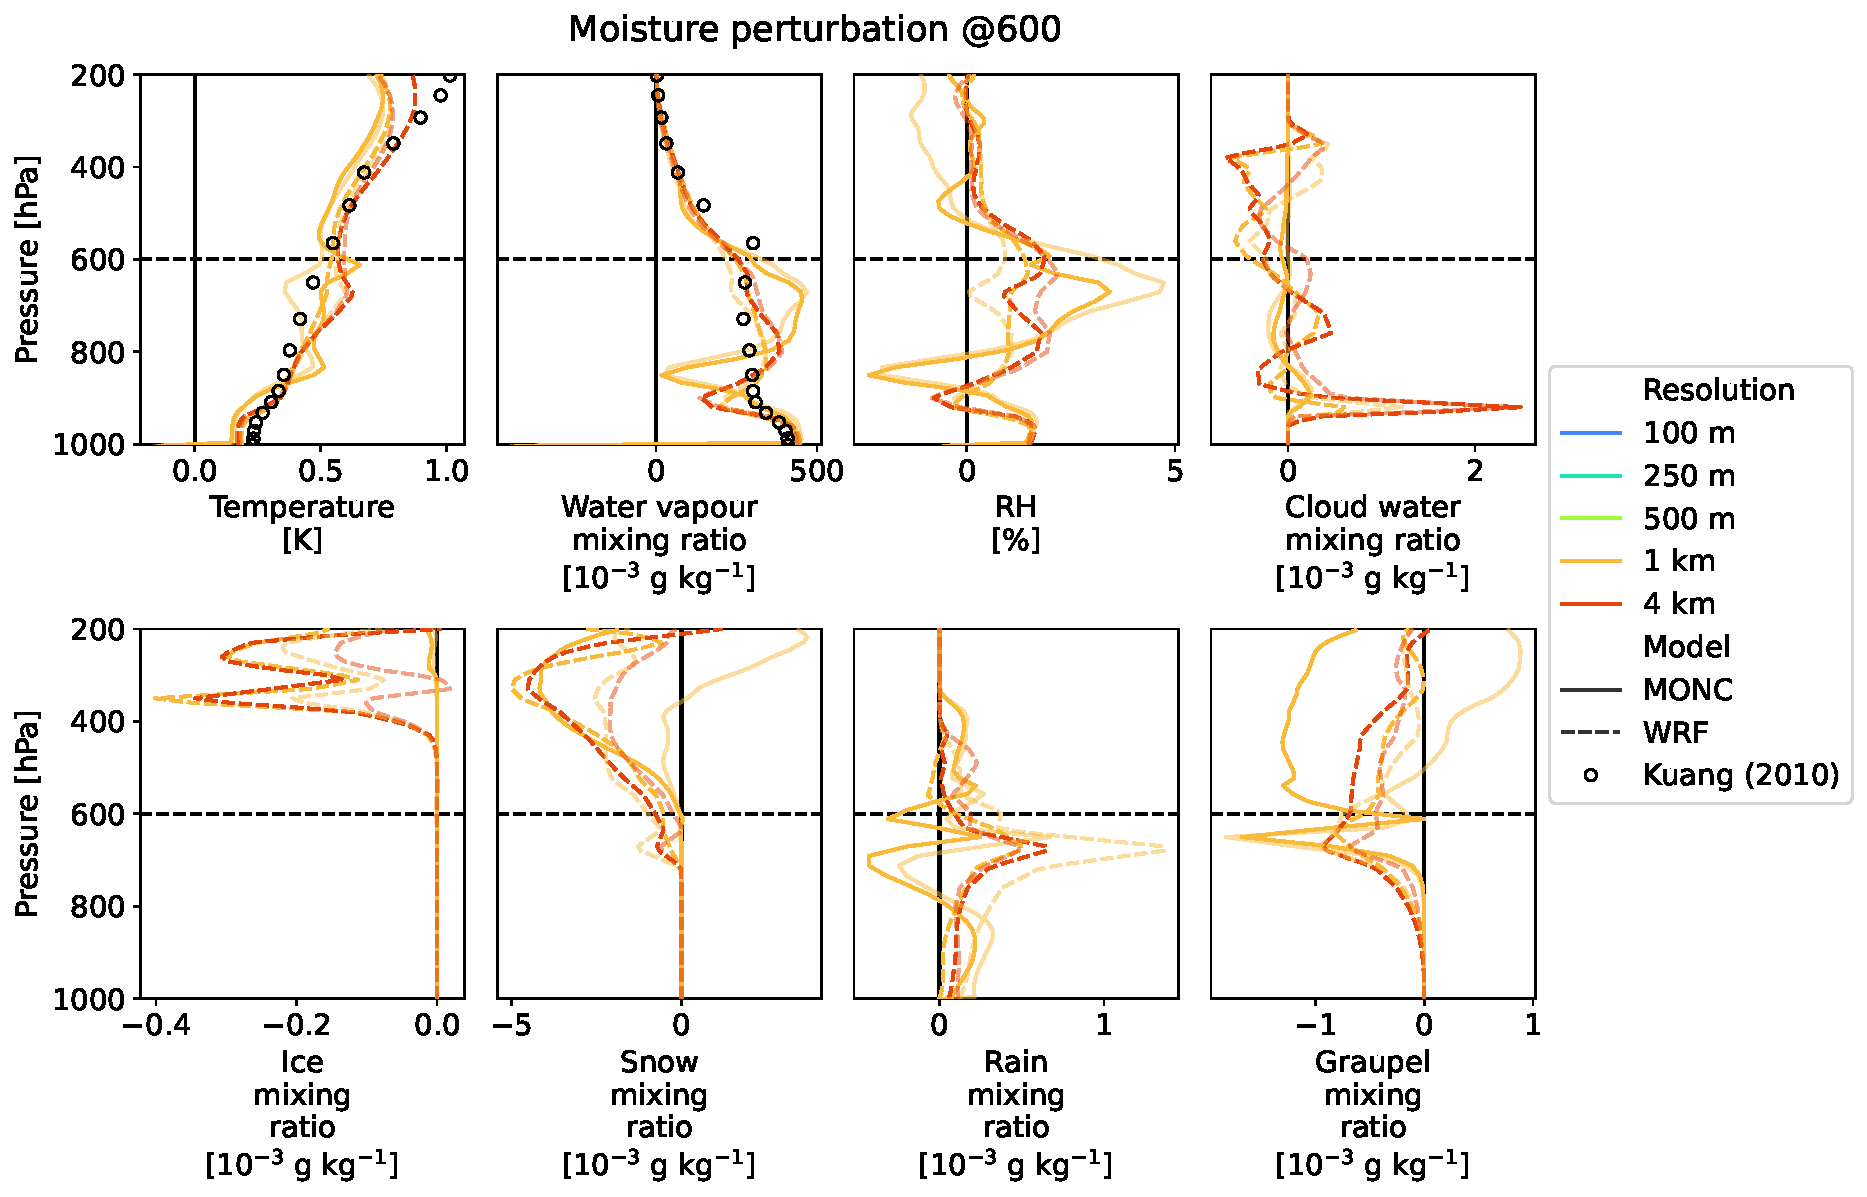
\includegraphics[width=\textwidth]{figures/pert_diffs_q_0.0002_@600}
    \caption{As in Figure \ref{fig:qpert_412}, but for a perturbation at 600
    hPa, and with black circles showing the responses of K10 to a specific
    humidity perturbation at 565 hPa.}
    \label{fig:qpert_600}
\end{figure}

\begin{figure}[pth]
    \noindent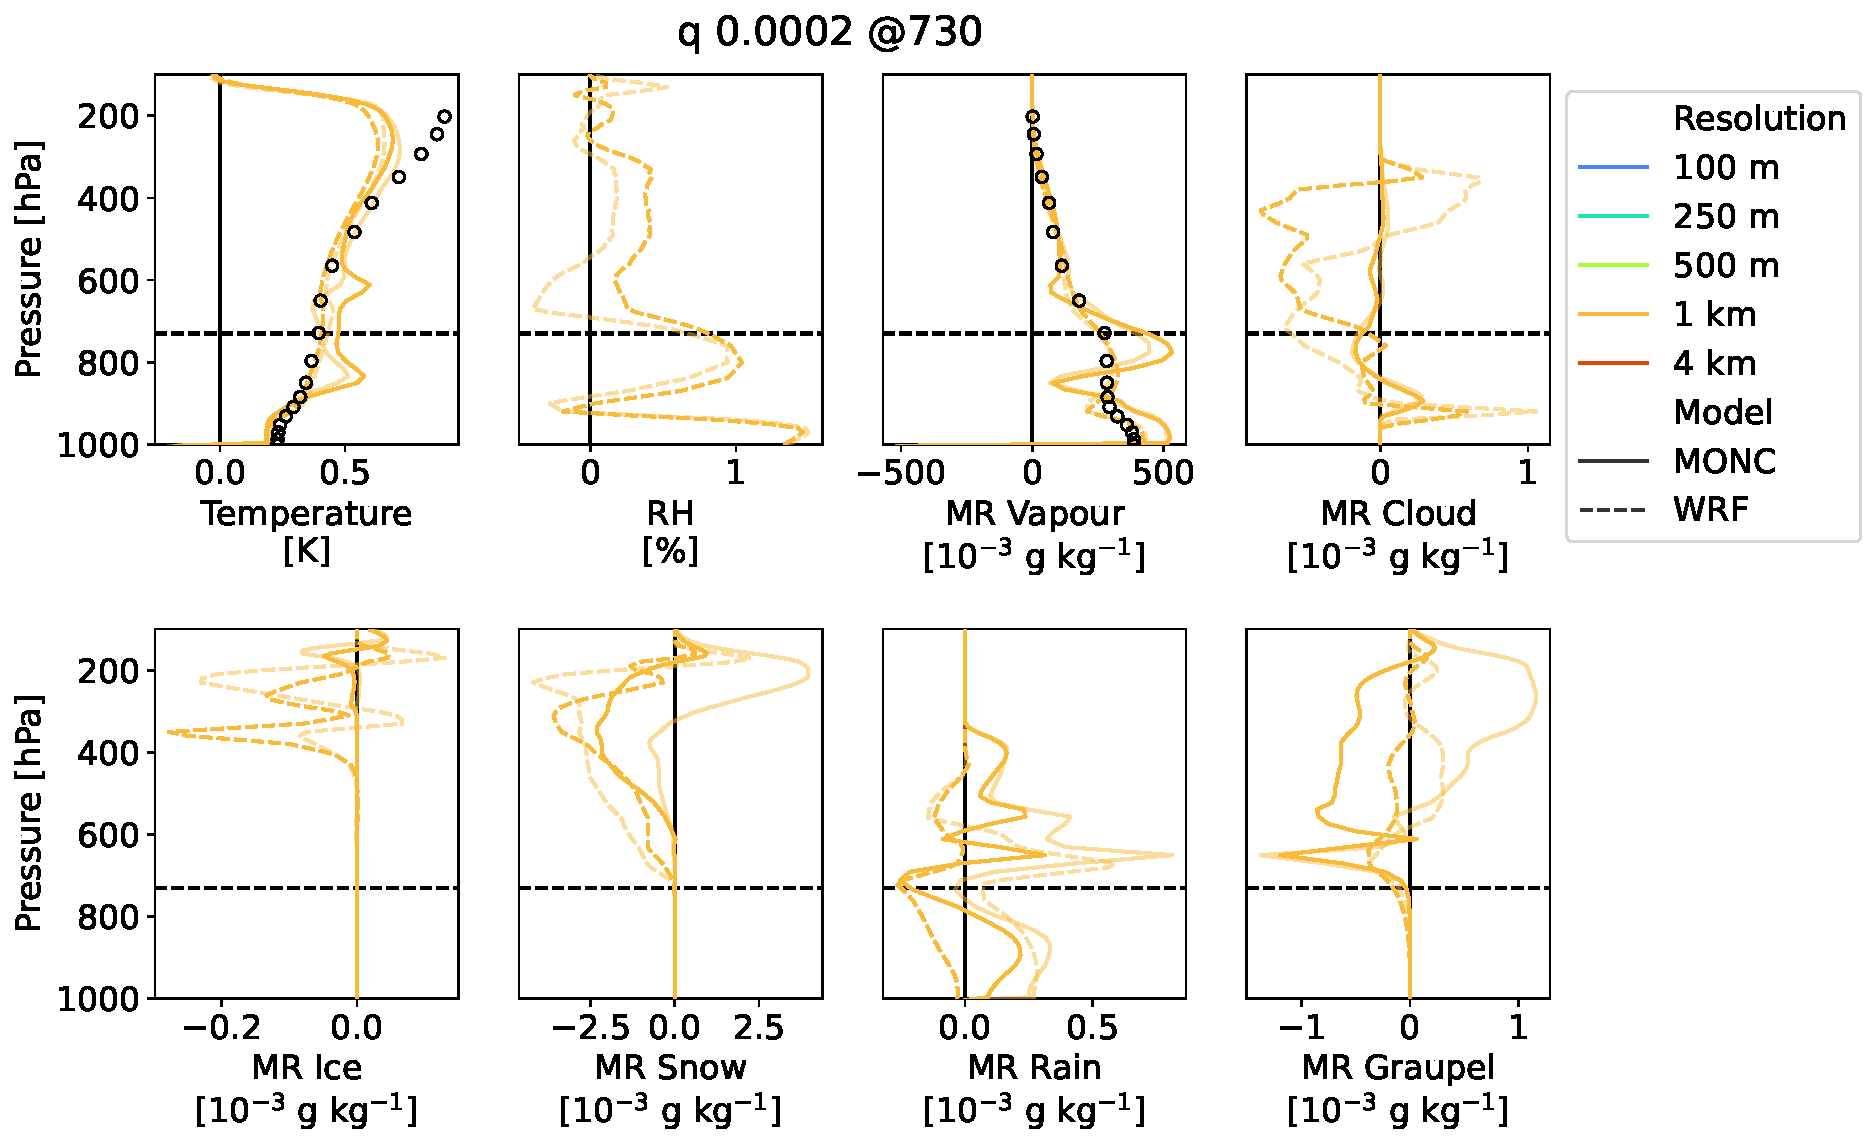
\includegraphics[width=\textwidth]{figures/pert_diffs_q_0.0002_@730}
    \caption{As in Figure \ref{fig:qpert_412}, but for a perturbation at 730
    hPa, and with black circles showing the responses of K10 to a specific
    humidity perturbation at 729 hPa.}
    \label{fig:qpert_730}
\end{figure}

\begin{figure}[pth]
    \noindent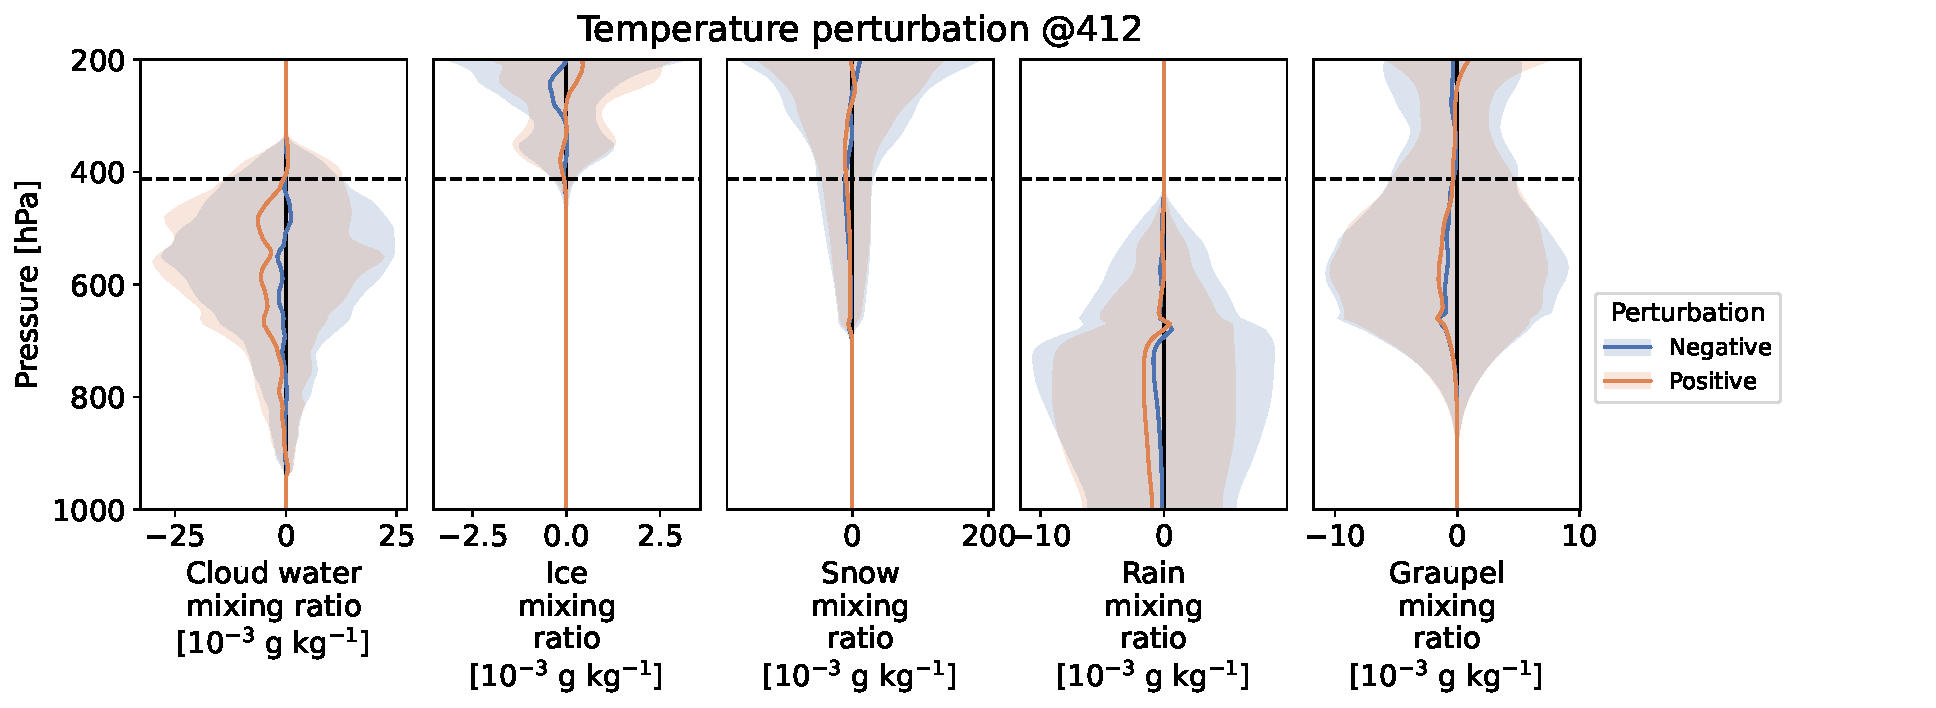
\includegraphics[width=\textwidth]{figures/pert_var_T_0.5_@412}
    \caption{Mean responses (solid line) and the $\pm$ 1 standard deviation
    range (shaded) for a temperature perturbation of $\pm$0.5 K at 412 hPa in
    the WRF runs at 100 m grid spacing. The solid vertical line shows zero
    response, the dashed horizontal line shows the level of maximum
    perturbation.}
    \label{fig:var_T_412}
\end{figure}

\begin{figure}[pth]
    \noindent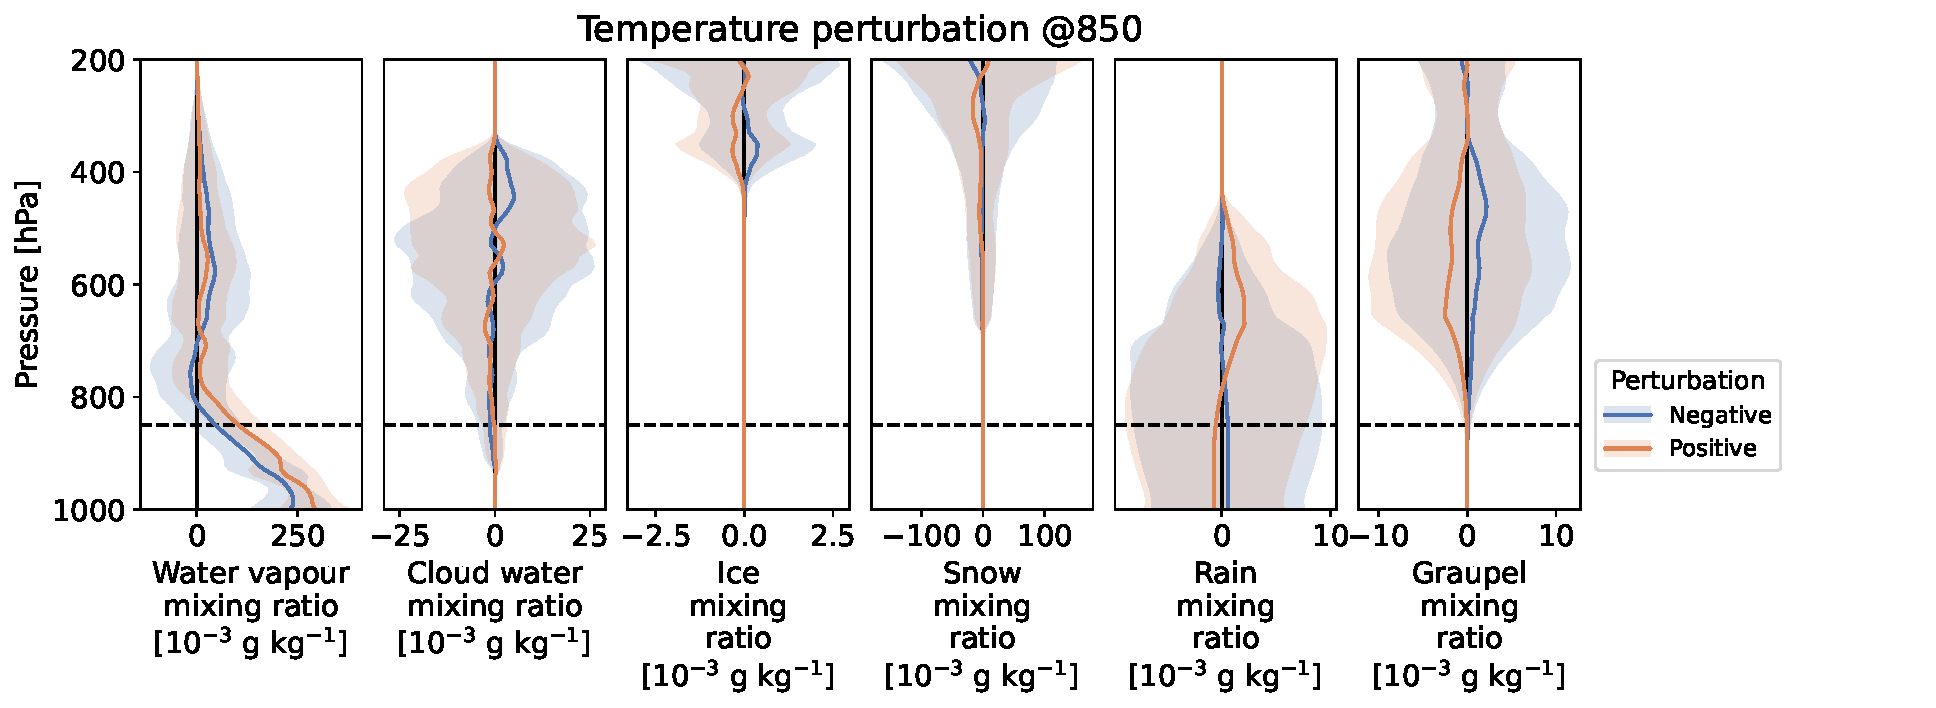
\includegraphics[width=\textwidth]{figures/pert_var_T_0.5_@850}
    \caption{As in Figure \ref{fig:var_T_412} but for a temperature perturbation
    at 850 hPa.}
    \label{fig:var_T_850}
\end{figure}

\begin{figure}[pth]
    \noindent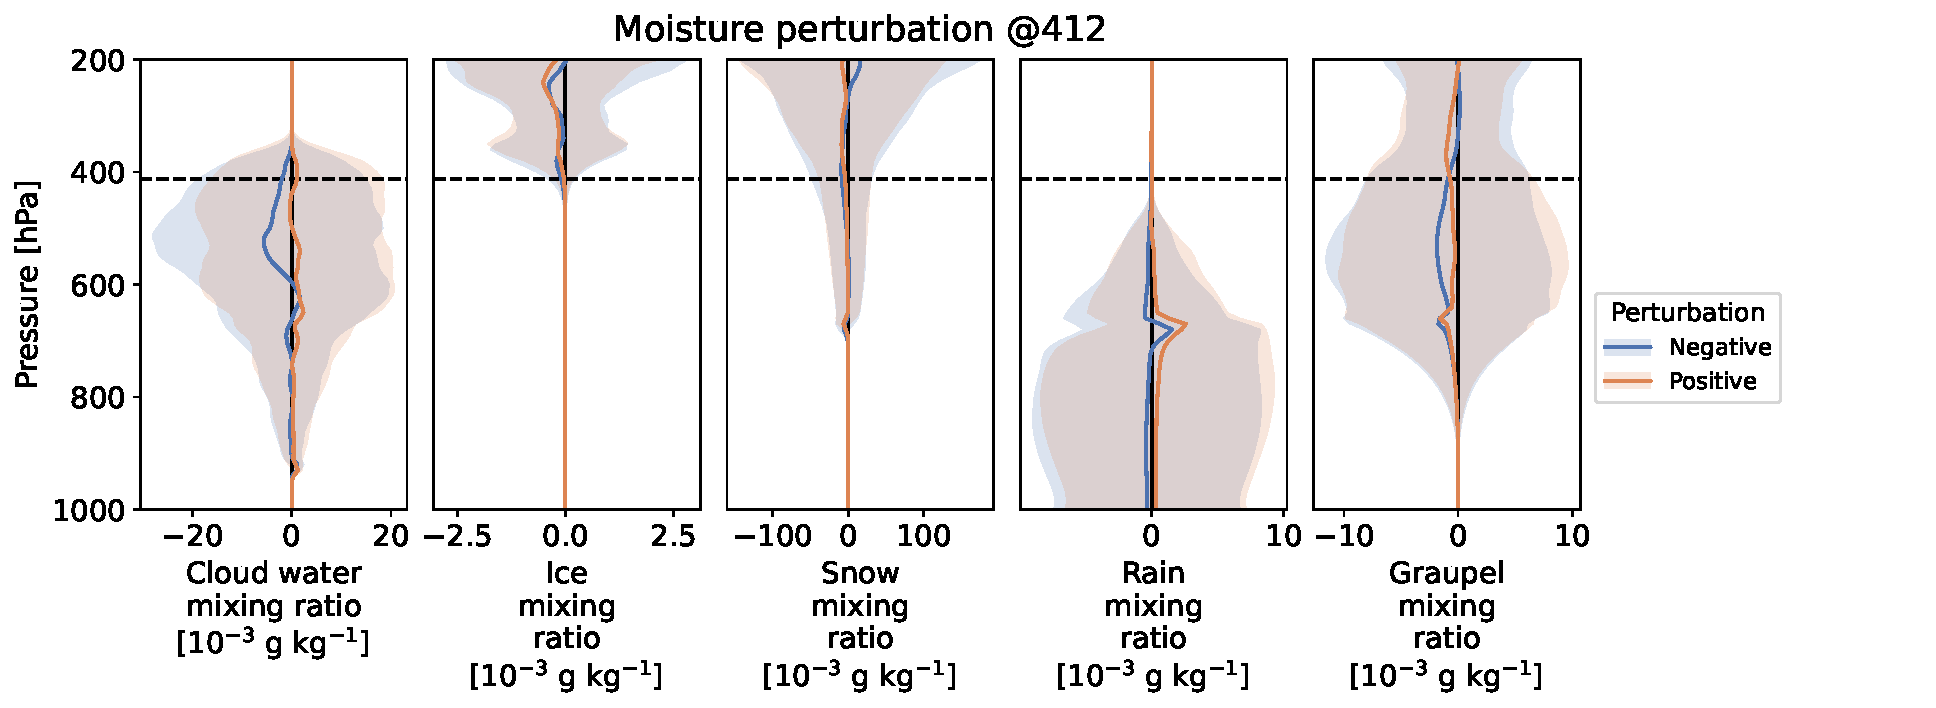
\includegraphics[width=\textwidth]{figures/pert_var_q_0.0002_@412}
    \caption{As in Figure \ref{fig:var_T_412} but for a water vapor mixing ratio
    perturbation of 0.2 g kg$^{-1}$ at 412 hPa.}
    \label{fig:var_q_412}
\end{figure}

\begin{figure}[pth]
    \noindent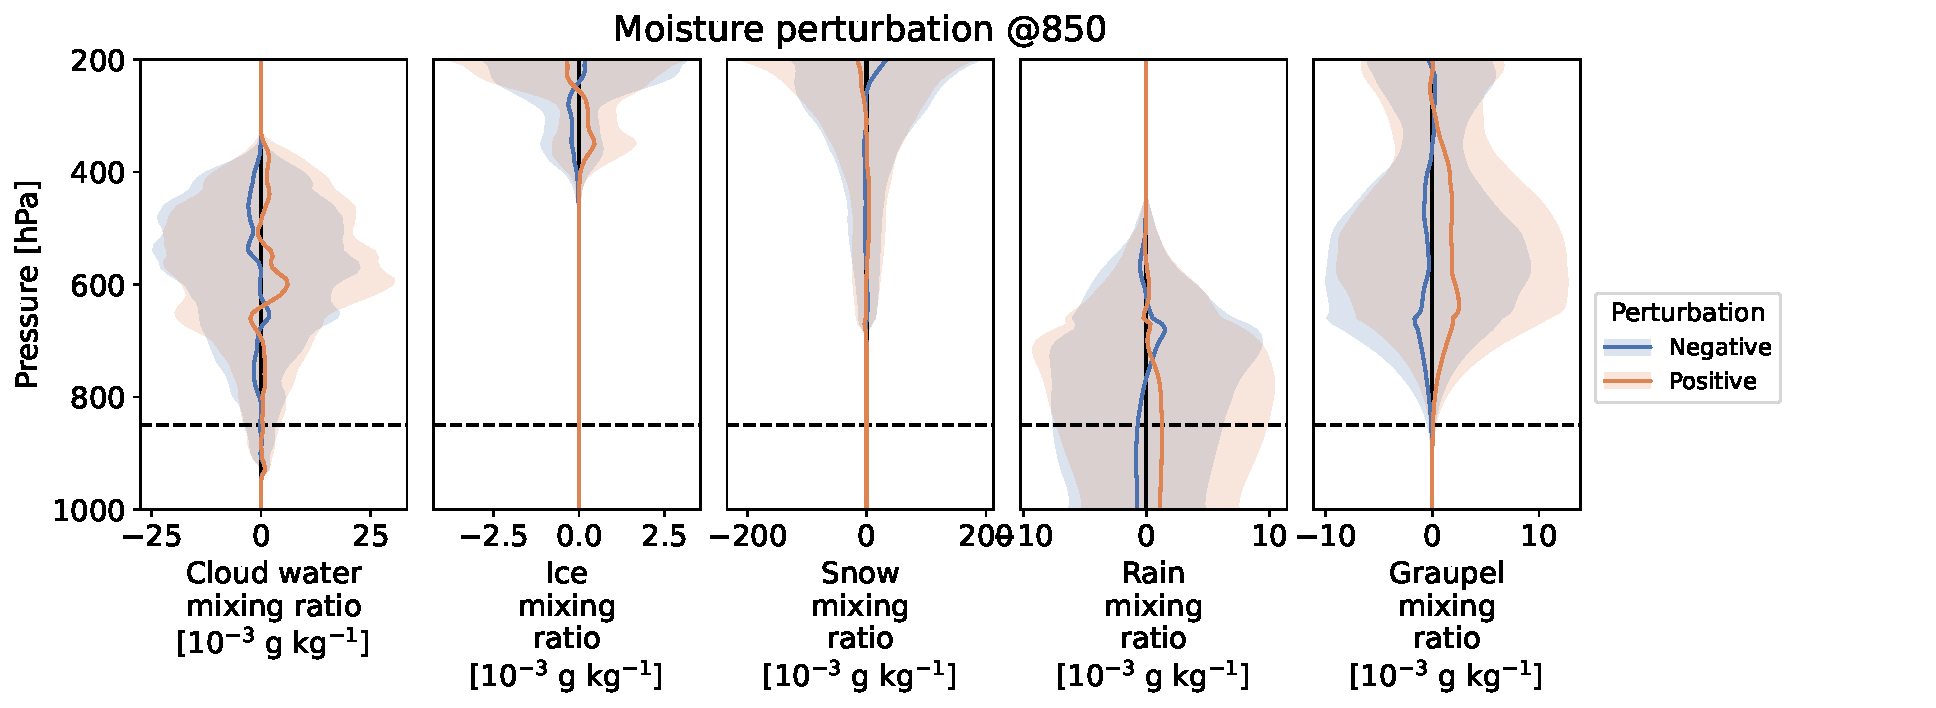
\includegraphics[width=\textwidth]{figures/pert_var_q_0.0002_@850}
    \caption{As in Figure \ref{fig:var_q_412} but for a water vapor mixing ratio
    perturbation of 0.2 g kg$^{-1}$ at 850 hPa.}
    \label{fig:var_q_850}
\end{figure}

\end{document}